\documentclass[10pt]{article}

% ============================================================
% PACKAGES
% ============================================================

\usepackage[a4paper,margin=0.65in]{geometry}
\usepackage{amsmath,amssymb}
\usepackage{graphicx}
\usepackage{booktabs}
\usepackage{array}
\usepackage{float}
\usepackage{hyperref}
\usepackage{enumitem}
\usepackage{xcolor}
\usepackage{tikz}
\usepackage{multirow}
\usepackage{caption}
\usepackage{subcaption}
\graphicspath{{./}}

\usetikzlibrary{
positioning,
arrows.meta,
shapes.geometric,
fit,
calc
}

% ============================================================
% FORMATTING
% ============================================================

\setlist{nosep,leftmargin=*}
\renewcommand{\arraystretch}{1.2}
\setlength{\parindent}{0pt}
\setlength{\parskip}{2pt}

\hypersetup{
    colorlinks=true,
    linkcolor=blue,
    urlcolor=blue,
    citecolor=blue
}

% ============================================================
% TIKZ STYLES
% ============================================================

\tikzset{
block/.style={
draw,
rounded corners,
minimum width=1.55cm,
minimum height=0.60cm,
align=center,
fill=blue!10,
font=\scriptsize
},
attn/.style={
draw,
rounded corners,
minimum width=1.55cm,
minimum height=0.60cm,
align=center,
fill=green!12,
font=\scriptsize
},
arrow/.style={
-{Latex[length=2mm]},
thin
}
}

% ============================================================
% DOCUMENT
% ============================================================

\begin{document}

% ============================================================
% TITLE
% ============================================================

\begin{center}

{\large\textbf{Shiv Nadar University Chennai}}\\[2mm]

{\normalsize\textbf{CS3807 -- Deep Learning Laboratory}}\\[2mm]

{\large\textbf{Experiments 8, 9}}\\[1mm]

{\normalsize
\textbf{
Effect of Attention Type and Attention Position\\
in a Pretrained ResNet50
}}

\end{center}

\vspace{3mm}

% ============================================================
% COURSE DETAILS
% ============================================================

\begin{center}
\begin{tabular}{|p{3.5cm}|p{8.7cm}|p{2.1cm}|}
\hline
\textbf{Degree \& Branch}
&
B.Tech Artificial Intelligence \& Data Science
&
Semester V
\\
\hline

\textbf{Subject Code \& Name}
&
CS3807 -- Deep Learning Laboratory
&
AY: 2026--27
\\
\hline

\textbf{Student Name \& Reg.\ No.}
&
\multicolumn{2}{p{10.9cm}|}{Guru Divya Darshini U \quad (Reg.\ No.\ 24011101032)}
\\
\hline
\end{tabular}
\end{center}

% ============================================================
\section*{1. Objective}
% ============================================================

The objective of this experiment is to understand how different attention
mechanisms modify a pretrained convolutional neural network and how the
\textbf{position at which attention is inserted} influences image
classification performance.

A single pretrained architecture,

\[
\boxed{\text{ResNet50 pretrained on ImageNet}}
\]

is used throughout the experiment.

Students will investigate:

\begin{itemize}

\item channel attention;

\item spatial attention;

\item sequential channel--spatial attention;

\item lightweight self-attention;

\item different positions for inserting attention within ResNet50;

\item single-stage and multi-stage attention;

\item attention ordering;

\item additional established attention mechanisms; and

\item qualitative interpretation using internal attention maps and Grad-CAM.

\end{itemize}

The experiment emphasizes that the effectiveness of attention depends not
only on the attention mechanism itself, but also on the characteristics of
the feature representation on which it operates.


\medskip
\fbox{\parbox{0.97\linewidth}{\small\textbf{Note on the results.} All numbers in the \emph{Observations} blocks of this document come from the executed notebook (\texttt{Attention\_ResNet50\_Lab\_1\_complete.ipynb}, Google Colab, T4 GPU, TensorFlow 2.21 / Keras 3.13). Every model was trained once with the same seed (42); the test split contains 551 images, so one accuracy value has a standard error of about 1.28 points (95\% interval $\pm2.5$ points). Differences smaller than this are \textbf{within noise for a single run} and are described as such.}}

\subsection*{Observations: Aim}
To study how the \emph{type} (channel, spatial, channel--spatial, self-attention, SE, ECA, CBAM, coordinate attention), the \emph{position} ($P_1$--$P_4$, single and multiple stages), the \emph{order} and the \emph{spatial kernel size} of attention modules inserted into an ImageNet-pretrained ResNet50 affect flower classification on \texttt{tf\_flowers}, and to combine quantitative results, computational cost, and qualitative evidence (internal attention maps and Grad-CAM).


% ============================================================
\section*{2. Learning Outcomes}
% ============================================================

After completing this experiment, students will be able to:

\begin{enumerate}

\item explain the stage-wise architecture of a pretrained ResNet50;

\item distinguish early, intermediate, and late convolutional features;

\item explain the motivation behind attention mechanisms;

\item implement channel attention;

\item implement spatial attention;

\item implement sequential channel--spatial attention;

\item implement a lightweight self-attention mechanism;

\item insert an attention module at different stages of a pretrained network;

\item analyze the influence of attention position;

\item compare different attention mechanisms under a controlled experimental
protocol;

\item analyze classification accuracy and class-wise performance;

\item visualize internal attention maps;

\item generate Grad-CAM explanations;

\item distinguish an internal attention map from a post-hoc explanation map;

\item analyze accuracy--complexity trade-offs; and

\item perform controlled ablation studies.

\end{enumerate}

% ============================================================
\section*{3. Dataset}
% ============================================================

\textbf{Recommended Dataset: TensorFlow Flowers (\texttt{tf\_flowers})}

The TensorFlow Flowers dataset contains natural RGB flower images belonging
to five classes:

\begin{center}
\texttt{daisy},
\quad
\texttt{dandelion},
\quad
\texttt{roses},
\quad
\texttt{sunflowers},
\quad
\texttt{tulips}.
\end{center}

The images contain variations in:

\begin{itemize}

\item scale;

\item viewpoint;

\item illumination;

\item background clutter;

\item flower size;

\item color;

\item texture; and

\item object location.

\end{itemize}

These variations make the dataset suitable for studying the behavior of
attention mechanisms.

% ============================================================
\subsection*{3.1 Image Preprocessing}
% ============================================================

Resize every input image to

\[
224\times224\times3.
\]

The image should be preprocessed using the preprocessing procedure expected
by the ImageNet-pretrained ResNet50.

Suitable data augmentation may include:

\begin{itemize}

\item random horizontal flipping;

\item small rotations;

\item random zoom;

\item random translation; and

\item mild contrast variation.

\end{itemize}

The same augmentation strategy must be maintained for all model comparisons.

% ============================================================
\subsection*{3.2 Dataset Split}
% ============================================================

Use the same training, validation, and testing split for every experiment:

\[
\boxed{
70\% : 15\% : 15\%
}
\]

for

\[
\text{Training : Validation : Testing}.
\]

The exact same samples should be retained in each subset for all ablation
experiments.

This is necessary to ensure that differences in performance are caused by
changes in the model rather than changes in the dataset split.


\subsection*{Observations: Dataset Description}
\texttt{tf\_flowers} contains 3{,}670 RGB images of five classes. All images were resized to $224\times224\times3$ and cached once. A fixed, stratified 70/15/15 split (seed 42) gives \textbf{2{,}569 training, 550 validation and 551 test images}, reused for all 17 experiments. The test split has 135 dandelion, 95 daisy, 120 tulips, 105 sunflowers and 96 roses images (class order of the dataset: dandelion, daisy, tulips, sunflowers, roses). Images vary strongly in scale, viewpoint, illumination, background clutter and flower size (Fig.~\ref{fig:samples}).
\begin{figure}[H]
\centering
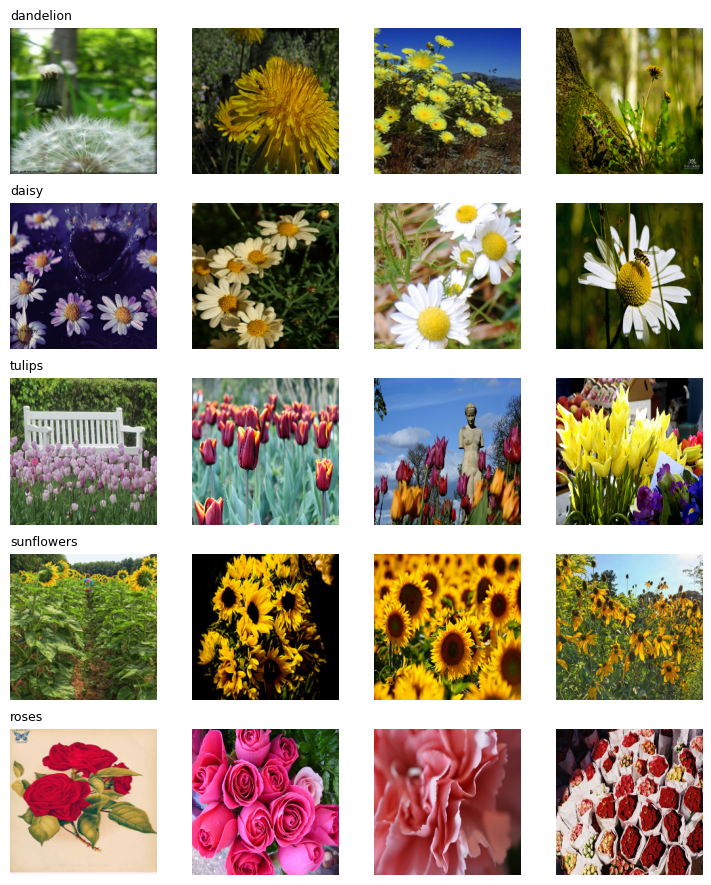
\includegraphics[width=0.55\linewidth]{figs/sample_images.png}
\caption{Sample training images of the five classes (4 per class).}
\label{fig:samples}
\end{figure}


% ============================================================
\section*{4. Pretrained Architecture: ResNet50}
% ============================================================

ResNet50 pretrained using ImageNet is used as the
\textbf{only backbone architecture} in this experiment.

For an input image

\[
I\in\mathbb{R}^{224\times224\times3},
\]

the major ResNet50 stages produce approximately the following feature
dimensions:

\begin{center}

\begin{tabular}{|l|c|c|}
\hline
\textbf{ResNet50 Stage}
&
\textbf{Spatial Resolution}
&
\textbf{Channels}
\\
\hline

Stem + MaxPool
&
$56\times56$
&
64
\\
\hline

conv2\_x
&
$56\times56$
&
256
\\
\hline

conv3\_x
&
$28\times28$
&
512
\\
\hline

conv4\_x
&
$14\times14$
&
1024
\\
\hline

conv5\_x
&
$7\times7$
&
2048
\\
\hline

\end{tabular}

\end{center}

As the network becomes deeper:

\[
\boxed{
\text{Spatial Resolution}\downarrow
}
\]

while

\[
\boxed{
\text{Feature Channels}\uparrow
}
\]

and the representation generally progresses from low-level visual
information toward higher-level semantic information.


\subsection*{Observations: ResNet50 Architecture}
\begin{table}[H]
\centering
\caption{Measured ResNet50 stage hierarchy (ImageNet weights, $224\times224\times3$ input). All four positions match the table of Section 7.}
\scriptsize
\resizebox{\textwidth}{!}{\begin{tabular}{l|ccccrl}
\toprule
\textbf{Stage} & \textbf{Position} & \textbf{Resolution} & \textbf{Channels} & \textbf{Residual blocks} & \textbf{Parameters} & \textbf{Level of features}\\
\midrule
Stem + MaxPool & -- & $56\times56$ & 64 & 0 & 9{,}728 & early: edges, colours, orientations\\
conv2\_x & $P_1$ & $56\times56$ & 256 & 3 & 220{,}032 & early: boundaries, textures\\
conv3\_x & $P_2$ & $28\times28$ & 512 & 4 & 1{,}230{,}336 & early/intermediate: local patterns\\
conv4\_x & $P_3$ & $14\times14$ & 1024 & 6 & 7{,}129{,}088 & intermediate: flower parts, shapes\\
conv5\_x & $P_4$ & $7\times7$ & 2048 & 3 & 14{,}998{,}528 & late: class-discriminative semantics\\
\bottomrule
\end{tabular}}
\end{table}

As depth increases the resolution falls from $56\times56$ to $7\times7$ while the channels rise from 256 to 2048. ResNet50 contains \textbf{16 residual (Add) connections} (3+4+6+3 bottleneck blocks); conv5\_x alone holds 14{,}998{,}528 of the 23{,}587{,}712 backbone parameters (about 64\%). The baseline (pretrained ResNet50 $\to$ global average pooling $\to$ Dropout 0.3 $\to$ Dense(5)) has \textbf{23{,}597{,}957} parameters, of which 10{,}245 belong to the new classification head.


% ============================================================
\section*{5. Understanding ResNet50 Feature Hierarchy}
% ============================================================

The approximate interpretation of different stages is:

\begin{itemize}

\item \textbf{Early features:}
edges, colors, orientations, boundaries, and simple textures.

\item \textbf{Intermediate features:}
local patterns, repeated structures, flower parts, petal arrangements, and
shape information.

\item \textbf{Late features:}
high-level object structures and class-discriminative semantic information.

\end{itemize}

Therefore, the same attention mechanism may produce different behavior when
inserted at different locations.

% ============================================================
\section*{6. Why Attention Position Matters}
% ============================================================

Attention is not independent of the features on which it operates.

Suppose an attention module receives

\[
F\in\mathbb{R}^{H\times W\times C}.
\]

The values of

\[
H,\qquad W,\qquad C
\]

and the semantic meaning of the feature tensor change significantly with
network depth.

Therefore:

\begin{itemize}

\item \textbf{early-stage attention} operates on high-resolution,
low-level visual information;

\item \textbf{middle-stage attention} operates on intermediate features
containing both spatial and semantic information; and

\item \textbf{late-stage attention} operates on low-resolution,
high-level semantic representations.

\end{itemize}

Thus, students should investigate both:

\[
\boxed{\text{Which attention mechanism should be used?}}
\]

and

\[
\boxed{\text{Where should the attention mechanism be inserted?}}
\]

% ============================================================
\section*{7. Candidate Attention Positions}
% ============================================================

Define four candidate attention positions in ResNet50.

\[
P_1:
\text{ after conv2\_x},
\]

\[
P_2:
\text{ after conv3\_x},
\]

\[
P_3:
\text{ after conv4\_x},
\]

\[
P_4:
\text{ after conv5\_x}.
\]

The corresponding feature dimensions are:

\begin{center}

\begin{tabular}{|c|c|c|c|}
\hline

\textbf{Position}
&
\textbf{Location}
&
\textbf{Resolution}
&
\textbf{Channels}
\\
\hline

$P_1$
&
After conv2\_x
&
$56\times56$
&
256
\\
\hline

$P_2$
&
After conv3\_x
&
$28\times28$
&
512
\\
\hline

$P_3$
&
After conv4\_x
&
$14\times14$
&
1024
\\
\hline

$P_4$
&
After conv5\_x
&
$7\times7$
&
2048
\\
\hline

\end{tabular}

\end{center}

For the principal laboratory exercise, students should concentrate on

\[
\boxed{
P_2,\quad P_3,\quad P_4
}
\]

because $P_1$ contains comparatively high-resolution features and may
substantially increase the computational cost of some attention mechanisms.

% ============================================================
\section*{8. Baseline Model}
% ============================================================

The baseline is the pretrained ResNet50 without any additional attention
mechanism.

\begin{center}

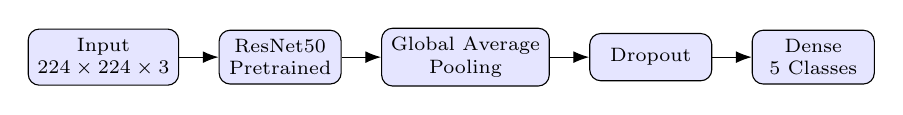
\begin{tikzpicture}[node distance=5mm]

\node[block] (a)
{Input\\$224\times224\times3$};

\node[block,right=of a] (b)
{ResNet50\\Pretrained};

\node[block,right=of b] (c)
{Global Average\\Pooling};

\node[block,right=of c] (d)
{Dropout};

\node[block,right=of d] (e)
{Dense\\5 Classes};

\foreach \x/\y in {a/b,b/c,c/d,d/e}
\draw[arrow] (\x)--(\y);

\end{tikzpicture}

\end{center}

The baseline establishes the reference performance against which the
attention-based models are compared.

% ============================================================
\section*{9. Channel Attention}
% ============================================================

Consider a feature tensor

\[
F\in\mathbb{R}^{H\times W\times C}.
\]

Channel attention determines the relative importance of different feature
channels.

Global average pooling is first used to generate a channel descriptor:

\[
z_c
=
\frac{1}{HW}
\sum_{i=1}^{H}
\sum_{j=1}^{W}
F(i,j,c).
\]

Thus,

\[
z\in\mathbb{R}^{C}.
\]

The channel descriptor is transformed using two learnable transformations:

\[
M_c(F)
=
\sigma
\left(
W_2
\delta
\left(
W_1z
\right)
\right),
\]

where:

\begin{itemize}

\item $\delta(\cdot)$ denotes a nonlinear activation such as ReLU;

\item $\sigma(\cdot)$ denotes the sigmoid activation;

\item $W_1$ reduces the channel representation; and

\item $W_2$ restores the channel dimension.

\end{itemize}

The refined feature tensor is:

\[
F_c
=
F\odot M_c(F).
\]

Channel attention attempts to answer:

\[
\boxed{\text{Which feature channels are important?}}
\]

A reduction ratio of

\[
r=16
\]

may be used as the default setting throughout the laboratory experiment.

The reduction ratio need not be treated as a separate mandatory ablation.

% ============================================================
\section*{10. Spatial Attention}
% ============================================================

Spatial attention determines the spatial regions that should receive greater
importance.

For the input feature tensor

\[
F\in\mathbb{R}^{H\times W\times C},
\]

compute average pooling across channels:

\[
F_{\mathrm{avg}}
=
\operatorname{Mean}_{c}(F),
\]

and maximum pooling across channels:

\[
F_{\mathrm{max}}
=
\operatorname{Max}_{c}(F).
\]

Both tensors have dimensions

\[
H\times W\times1.
\]

Concatenate them:

\[
F_s
=
[
F_{\mathrm{avg}}
\Vert
F_{\mathrm{max}}
].
\]

The spatial attention map is then computed as

\[
M_s(F)
=
\sigma
\left(
\operatorname{Conv}_{7\times7}(F_s)
\right).
\]

Therefore,

\[
M_s(F)
\in
\mathbb{R}^{H\times W\times1}.
\]

The spatially refined feature is

\[
F_s'
=
F\odot M_s(F).
\]

Spatial attention answers:

\[
\boxed{\text{Which spatial locations are important?}}
\]

% ============================================================
\section*{11. Sequential Channel--Spatial Attention}
% ============================================================

Channel and spatial attention can be sequentially applied.

First,

\[
F_c
=
M_c(F)\odot F.
\]

Then,

\[
F_{cs}
=
M_s(F_c)\odot F_c.
\]

The overall structure becomes:

\[
\boxed{
F
\rightarrow
\text{Channel Attention}
\rightarrow
\text{Spatial Attention}
\rightarrow
F_{cs}
}
\]

This arrangement first determines

\[
\text{``what is important''}
\]

and then determines

\[
\text{``where it is important.''}
\]

A simplified diagram is shown below.

\begin{center}

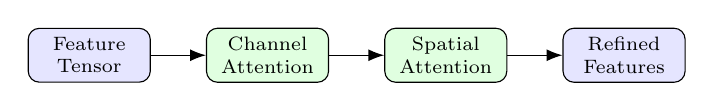
\begin{tikzpicture}[node distance=7mm]

\node[block] (a)
{Feature\\Tensor};

\node[attn,right=of a] (b)
{Channel\\Attention};

\node[attn,right=of b] (c)
{Spatial\\Attention};

\node[block,right=of c] (d)
{Refined\\Features};

\draw[arrow] (a)--(b);
\draw[arrow] (b)--(c);
\draw[arrow] (c)--(d);

\end{tikzpicture}

\end{center}

% ============================================================
\section*{12. Self-Attention}
% ============================================================

Self-attention allows spatial locations to interact directly with other
spatial locations.

For

\[
F\in\mathbb{R}^{H\times W\times C},
\]

flatten the spatial dimensions:

\[
X\in\mathbb{R}^{N\times C},
\]

where

\[
N=HW.
\]

Generate the query, key, and value matrices:

\[
Q=XW_Q,
\]

\[
K=XW_K,
\]

and

\[
V=XW_V.
\]

The attention matrix is

\[
A
=
\operatorname{softmax}
\left(
\frac{QK^T}{\sqrt{d}}
\right),
\]

where $d$ is the dimension of the query/key representation.

The attended output is

\[
Y=AV.
\]

After reshaping the output back to the original spatial structure, a residual
formulation may be used:

\[
F_{\mathrm{SA}}
=
F
+
\gamma
\operatorname{reshape}(Y),
\]

where $\gamma$ is a learnable scaling parameter.

Self-attention attempts to answer:

\[
\boxed{
\text{Which spatial features are related to other spatial features?}
}
\]

Since the attention matrix has dimension approximately

\[
N\times N,
\]

its computational requirements increase rapidly as

\[
N=HW
\]

increases.

Therefore, self-attention should preferably be introduced at

\[
P_3
\]

or

\[
P_4.
\]

% ============================================================
\section*{13. Inserting Attention into ResNet50}
% ============================================================

For any selected stage $P_k$, the network structure can be written as

\[
\text{Previous ResNet Stage}
\rightarrow
\text{Attention}
\rightarrow
\text{Next ResNet Stage}.
\]

For example, attention inserted after conv4\_x gives:

\[
\boxed{
\text{conv4\_x}
\rightarrow
\text{Attention}
\rightarrow
\text{conv5\_x}
}
\]

For channel--spatial attention:

\[
\boxed{
\text{conv4\_x}
\rightarrow
\text{Channel Attention}
\rightarrow
\text{Spatial Attention}
\rightarrow
\text{conv5\_x}
}
\]

The student must record the feature dimensions immediately before and after
the attention block.

Attention should not unintentionally modify the spatial or channel
dimensions unless the selected mechanism explicitly requires such a
transformation.


\subsection*{Observations: Attention Mechanisms and Proposed Experimental Architecture}
Each module takes $F\in\mathbb{R}^{H\times W\times C}$ and returns a tensor of the same shape; it is inserted between two ResNet stages (``previous stage $\to$ attention $\to$ next stage'').
\begin{itemize}
\item \textbf{Channel attention (= SE):} GAP $\to$ Dense($C/16$, ReLU) $\to$ Dense($C$, sigmoid), gating $F$ channel-wise. Because the PDF formulation is identical to SE, it is reported as ``Channel / SE''.
\item \textbf{Spatial attention:} channel-wise mean and max maps $\to$ $7\times7$ convolution $\to$ sigmoid (99 parameters).
\item \textbf{Channel$\to$Spatial:} the two above applied sequentially; \textbf{Spatial$\to$Channel} reverses the order.
\item \textbf{Self-attention:} $Q=XW_Q$, $K=XW_K$ with $d=C/8$, $V=XW_V$, $A=\mathrm{softmax}(QK^\top/\sqrt d)$, output $F+\gamma\,\mathrm{reshape}(AV)$ with $\gamma$ initialised to 0.
\item \textbf{Combined (A5):} Channel$\to$Spatial$\to$Self-attention.
\item \textbf{ECA:} 1-D convolution over the channel descriptor with adaptive kernel size ($k=5$ at $C=1024$), 5 parameters.
\item \textbf{CBAM:} channel gate from average- and max-pooled descriptors through a shared MLP, followed by a $7\times7$ spatial gate.
\item \textbf{Coordinate attention:} direction-aware pooling along $H$ and $W$ with a shared $1\times1$ transform.
\end{itemize}
\begin{table}[H]
\centering
\caption{Observation 1 -- feature dimensions immediately before and after the attention block (none of the modules changes $H$, $W$ or $C$).}
\scriptsize
\resizebox{\textwidth}{!}{\begin{tabular}{l|ccc}
\toprule
\textbf{Models} & \textbf{Position} & \textbf{Input to attention} & \textbf{Output of attention}\\
\midrule
A1/A2/A3/A4/A5, D1, E1, E2, F1, F2, F3 (single $P_3$ module) & $P_3$ & $14\times14\times1024$ & $14\times14\times1024$\\
B1 & $P_1$ & $56\times56\times256$ & $56\times56\times256$\\
B2 (and C2) & $P_2$ & $28\times28\times512$ & $28\times28\times512$\\
B4 (and C1, C2) & $P_4$ & $7\times7\times2048$ & $7\times7\times2048$\\
\bottomrule
\end{tabular}}
\end{table}

\begin{table}[H]
\centering
\caption{Registry of the 17 trained models.}
\scriptsize
\resizebox{\textwidth}{!}{\begin{tabular}{l|lll}
\toprule
\textbf{ID} & \textbf{Attention} & \textbf{Position(s)} & \textbf{Notes}\\
\midrule
A0 & none & -- & pretrained ResNet50 $\to$ GAP $\to$ Dropout $\to$ Dense(5)\\
A1 & Channel (= SE) & $P_3$ & GAP, FC(C/16), ReLU, FC(C), sigmoid\\
A2 & Spatial & $P_3$ & mean/max over channels, $7\times7$ conv, sigmoid\\
A3 (= B3) & Channel$\to$Spatial & $P_3$ & selected model\\
A4 & Self-attention & $P_3$ & $Q,K$ with $d=C/8$, $V$ with $C$, learnable residual $\gamma$ (init.\ 0)\\
A5 & Channel$\to$Spatial$\to$Self-attn & $P_3$ & combined\\
B1, B2, B4 & Channel$\to$Spatial & $P_1$, $P_2$, $P_4$ & position ablation\\
C1, C2 & Channel$\to$Spatial & $P_3{+}P_4$; $P_2{+}P_3{+}P_4$ & multi-stage\\
D1 & Spatial$\to$Channel & $P_3$ & order ablation\\
E1, E2 & Channel$\to$Spatial & $P_3$ & spatial kernel $k=3$, $k=5$ ($k=7$ is A3)\\
F1 & ECA & $P_3$ & adaptive 1-D kernel ($k=5$ at $C=1024$), 5 parameters\\
F2 & CBAM & $P_3$ & avg+max shared MLP channel gate, then $7\times7$ spatial gate\\
F3 & Coordinate Attention & $P_3$ & direction-aware pooling along $H$ and $W$\\
\bottomrule
\end{tabular}}
\end{table}



% ============================================================
\section*{14. Main Experiment 1: Attention-Type Ablation}
% ============================================================

The first experiment studies the effect of different types of attention.

Fix the attention position at

\[
\boxed{
P_3=\text{after conv4\_x}
}
\]

for all models.

Compare the following:

\begin{center}

\begin{tabular}{|l|c|c|c|}
\hline

\textbf{Model}
&
\textbf{Channel}
&
\textbf{Spatial}
&
\textbf{Self-Attention}
\\
\hline

A0: Baseline ResNet50
&
--
&
--
&
--
\\
\hline

A1: Channel Attention
&
$\checkmark$
&
--
&
--
\\
\hline

A2: Spatial Attention
&
--
&
$\checkmark$
&
--
\\
\hline

A3: Channel+Spatial
&
$\checkmark$
&
$\checkmark$
&
--
\\
\hline

A4: Self-Attention
&
--
&
--
&
$\checkmark$
\\
\hline

A5: Combined Attention
&
$\checkmark$
&
$\checkmark$
&
$\checkmark$
\\
\hline

\end{tabular}

\end{center}

This experiment investigates:

\[
\boxed{
\text{How does attention type affect model performance?}
}
\]

Students must keep the following identical:

\begin{itemize}

\item dataset split;

\item preprocessing;

\item augmentation;

\item optimizer;

\item learning rate schedule;

\item epochs;

\item batch size;

\item backbone;

\item classifier;

\item attention position; and

\item evaluation procedure.

\end{itemize}


\subsection*{Observations: Attention-Type Ablation (Experiment 1)}
\begin{table}[H]
\centering
\caption{Experiment 1 -- attention-type ablation at $P_3$ (test split, 551 images).}
\scriptsize
\resizebox{\textwidth}{!}{\begin{tabular}{l|cccc|rr|ccc}
\toprule
\textbf{Model} & \textbf{Acc.} & \textbf{Prec.} & \textbf{Recall} & \textbf{Macro F1} & \textbf{Total params} & \textbf{Attn params} & \textbf{Inf.\ ms/img} & \textbf{GFLOPs} & \textbf{Train min}\\
\midrule
A0 Baseline & 0.9002 & 0.9116 & 0.9026 & 0.9033 & 23{,}597{,}957 & 0 & 8.08 & 7.75 & 3.6\\
A1 Channel (SE) & 0.9129 & 0.9159 & 0.9105 & 0.9123 & 23{,}730{,}117 & 132{,}160 & 8.06 & 7.75 & 3.7\\
A2 Spatial & 0.9419 & 0.9453 & 0.9396 & 0.9419 & 23{,}598{,}056 & 99 & 8.17 & 7.75 & 3.7\\
A3 Channel+Spatial & 0.9437 & 0.9469 & 0.9389 & 0.9420 & 23{,}730{,}216 & 132{,}259 & 8.37 & 7.75 & 3.8\\
A4 Self-Attention & 0.9419 & 0.9432 & 0.9400 & 0.9412 & 24{,}908{,}678 & 1{,}310{,}721 & 7.62 & 8.35 & 4.1\\
A5 Combined (C+S+SA) & 0.9274 & 0.9347 & 0.9237 & 0.9266 & 25{,}040{,}937 & 1{,}442{,}980 & 7.93 & 8.36 & 4.4\\
\bottomrule
\end{tabular}}
\end{table}

Relative to the baseline (accuracy 0.9002, macro F1 0.9033):
\begin{itemize}
\item \textbf{Spatial (A2), Channel$\to$Spatial (A3) and Self-attention (A4)} give the clearest gains: $+4.2$, $+4.4$ and $+4.2$ accuracy points ($+3.9$, $+3.9$, $+3.8$ macro-F1 points), each beyond the $\pm2.5$-point interval. A2, A3 and A4 are practically tied with each other.
\item \textbf{Channel/SE (A1)} gives only $+1.3$ points, which is within noise.
\item \textbf{Combined (A5)} reaches 0.9274 ($+2.7$ points), \emph{lower} than A3 and A4 although it contains both: more attention in one place is not better here.
\end{itemize}
The A2 result is notable: a spatial module with \textbf{99 parameters} matches self-attention with 1{,}310{,}721 parameters. Sections 28 and 29 show why this gain should be interpreted cautiously.


% ============================================================
\section*{15. Main Experiment 2: Attention-Position Ablation}
% ============================================================

The second experiment investigates the influence of the position of
attention.

Fix the attention type as:

\[
\boxed{
\text{Channel Attention}
\rightarrow
\text{Spatial Attention}
}
\]

and insert exactly the same module at different stages.

\begin{center}

\begin{tabular}{|l|l|c|c|}
\hline

\textbf{Experiment}
&
\textbf{Attention Position}
&
\textbf{Resolution}
&
\textbf{Channels}
\\
\hline

B1
&
After conv2\_x
&
$56\times56$
&
256
\\
\hline

B2
&
After conv3\_x
&
$28\times28$
&
512
\\
\hline

B3
&
After conv4\_x
&
$14\times14$
&
1024
\\
\hline

B4
&
After conv5\_x
&
$7\times7$
&
2048
\\
\hline

\end{tabular}

\end{center}

Students should study whether attention is more beneficial for:

\begin{itemize}

\item high-resolution low-level features;

\item intermediate representations; or

\item low-resolution semantic features.

\end{itemize}

The principal question is:

\[
\boxed{
\text{How does the location of attention influence performance?}
}
\]


\subsection*{Observations: Attention-Position Ablation (Experiment 2)}
\begin{table}[H]
\centering
\caption{Experiment 2 -- Channel$\to$Spatial attention at $P_1$ (B1), $P_2$ (B2), $P_3$ (B3 = A3) and $P_4$ (B4).}
\scriptsize
\resizebox{\textwidth}{!}{\begin{tabular}{l|cccc|rr|ccc}
\toprule
\textbf{Model} & \textbf{Acc.} & \textbf{Prec.} & \textbf{Recall} & \textbf{Macro F1} & \textbf{Total params} & \textbf{Attn params} & \textbf{Inf.\ ms/img} & \textbf{GFLOPs} & \textbf{Train min}\\
\midrule
B1 C+S @ $P_1$ & 0.9129 & 0.9201 & 0.9110 & 0.9119 & 23{,}606{,}520 & 8{,}563 & 8.16 & 7.76 & 5.3\\
B2 C+S @ $P_2$ & 0.9328 & 0.9349 & 0.9315 & 0.9326 & 23{,}631{,}368 & 33{,}411 & 8.03 & 7.75 & 4.5\\
A3 Channel+Spatial & 0.9437 & 0.9469 & 0.9389 & 0.9420 & 23{,}730{,}216 & 132{,}259 & 8.37 & 7.75 & 3.8\\
B4 C+S @ $P_4$ & 0.9365 & 0.9361 & 0.9378 & 0.9351 & 24{,}124{,}520 & 526{,}563 & 7.87 & 7.75 & 3.5\\
\bottomrule
\end{tabular}}
\end{table}

$P_3$ is best (0.9437 / 0.9420), followed by $P_4$ (0.9365), $P_2$ (0.9328) and $P_1$ (0.9129, only $+1.3$ points over the baseline). The $P_2$--$P_4$ differences are about one standard error, so only two statements are supported: attention at the high-resolution $P_1$ is clearly less useful than at $P_3$ ($-3.1$ points) and also costs the most (5.3 min estimated training time versus 3.8 min at $P_3$), and intermediate/late positions work at least as well as each other. Attention parameters grow with channel width ($8{,}563$ at $P_1$, $33{,}411$ at $P_2$, $132{,}259$ at $P_3$, $526{,}563$ at $P_4$) since the channel MLP scales with $C^2$.

% ============================================================
\section*{16. Main Experiment 3: Multiple Attention Positions}
% ============================================================

Attention may also be inserted at more than one ResNet50 stage.

Compare:

\[
\text{Attention only at }P_3,
\]

\[
\text{Attention only at }P_4,
\]

and

\[
\text{Attention at }P_3+P_4.
\]

As an extended experiment, students may evaluate:

\[
P_2+P_3+P_4.
\]

The purpose is to investigate whether applying attention repeatedly provides
sufficient performance improvement to justify the additional:

\begin{itemize}

\item parameters;

\item computation;

\item memory;

\item training time; and

\item inference time.

\end{itemize}

Students should experimentally answer:

\[
\boxed{
\text{Is attention at more locations necessarily more effective?}
}
\]


\subsection*{Observations: Multiple Attention Positions (Experiment 3)}
\begin{table}[H]
\centering
\caption{Experiment 3 -- single versus multiple attention positions (Channel$\to$Spatial).}
\scriptsize
\resizebox{\textwidth}{!}{\begin{tabular}{l|cccc|rr|ccc}
\toprule
\textbf{Model} & \textbf{Acc.} & \textbf{Prec.} & \textbf{Recall} & \textbf{Macro F1} & \textbf{Total params} & \textbf{Attn params} & \textbf{Inf.\ ms/img} & \textbf{GFLOPs} & \textbf{Train min}\\
\midrule
A3 Channel+Spatial & 0.9437 & 0.9469 & 0.9389 & 0.9420 & 23{,}730{,}216 & 132{,}259 & 8.37 & 7.75 & 3.8\\
B4 C+S @ $P_4$ & 0.9365 & 0.9361 & 0.9378 & 0.9351 & 24{,}124{,}520 & 526{,}563 & 7.87 & 7.75 & 3.5\\
C1 C+S @ $P_3{+}P_4$ & 0.9292 & 0.9279 & 0.9306 & 0.9286 & 24{,}256{,}779 & 658{,}822 & 7.81 & 7.75 & 3.9\\
C2 C+S @ $P_2{+}P_3{+}P_4$ & 0.9074 & 0.9147 & 0.9108 & 0.9079 & 24{,}290{,}190 & 692{,}233 & 8.41 & 7.76 & 4.7\\
\bottomrule
\end{tabular}}
\end{table}

Applying attention at more stages \textbf{did not help}: $P_3{+}P_4$ is 1.5 accuracy points below $P_3$ alone, and $P_2{+}P_3{+}P_4$ is 3.6 points below, while adding 526{,}563 and 559{,}974 attention parameters, and increasing estimated training time from 3.8 to 3.9 and 4.7 min. The three-stage model also shows a large train--validation gap (0.0825 versus 0.0412 for A3). The answer to ``Is attention at more locations necessarily more effective?'' is therefore \emph{no}.

% ============================================================
\section*{17. Main Experiment 4: Attention Order}
% ============================================================

The sequence in which channel and spatial attention are applied may influence
the resulting features.

Compare:

\[
\boxed{
\text{Channel}
\rightarrow
\text{Spatial}
}
\]

against

\[
\boxed{
\text{Spatial}
\rightarrow
\text{Channel}
}
\]

while maintaining the same insertion position.

For example, at $P_3$:

\[
F
\rightarrow
M_c
\rightarrow
M_s
\]

should be compared with

\[
F
\rightarrow
M_s
\rightarrow
M_c.
\]

Students should determine whether selecting informative feature channels
before selecting spatial regions produces behavior different from selecting
spatial regions first.


\subsection*{Observations: Attention Order (Experiment 4)}
\begin{table}[H]
\centering
\caption{Experiment 4 -- attention order at $P_3$.}
\scriptsize
\resizebox{\textwidth}{!}{\begin{tabular}{l|cccc|rr|ccc}
\toprule
\textbf{Model} & \textbf{Acc.} & \textbf{Prec.} & \textbf{Recall} & \textbf{Macro F1} & \textbf{Total params} & \textbf{Attn params} & \textbf{Inf.\ ms/img} & \textbf{GFLOPs} & \textbf{Train min}\\
\midrule
A3 Channel+Spatial & 0.9437 & 0.9469 & 0.9389 & 0.9420 & 23{,}730{,}216 & 132{,}259 & 8.37 & 7.75 & 3.8\\
D1 Spatial$\to$Channel & 0.9328 & 0.9306 & 0.9338 & 0.9319 & 23{,}730{,}216 & 132{,}259 & 7.97 & 7.75 & 3.8\\
\bottomrule
\end{tabular}}
\end{table}

Channel$\to$Spatial is 1.1 points better than Spatial$\to$Channel (0.9437 vs 0.9328), which is below two standard errors: \textbf{no reliable order effect}. The spatial maps of the two orders are very similar (per-image correlation 0.93--0.99, Fig.~\ref{fig:order}).
\begin{figure}[H]
\centering
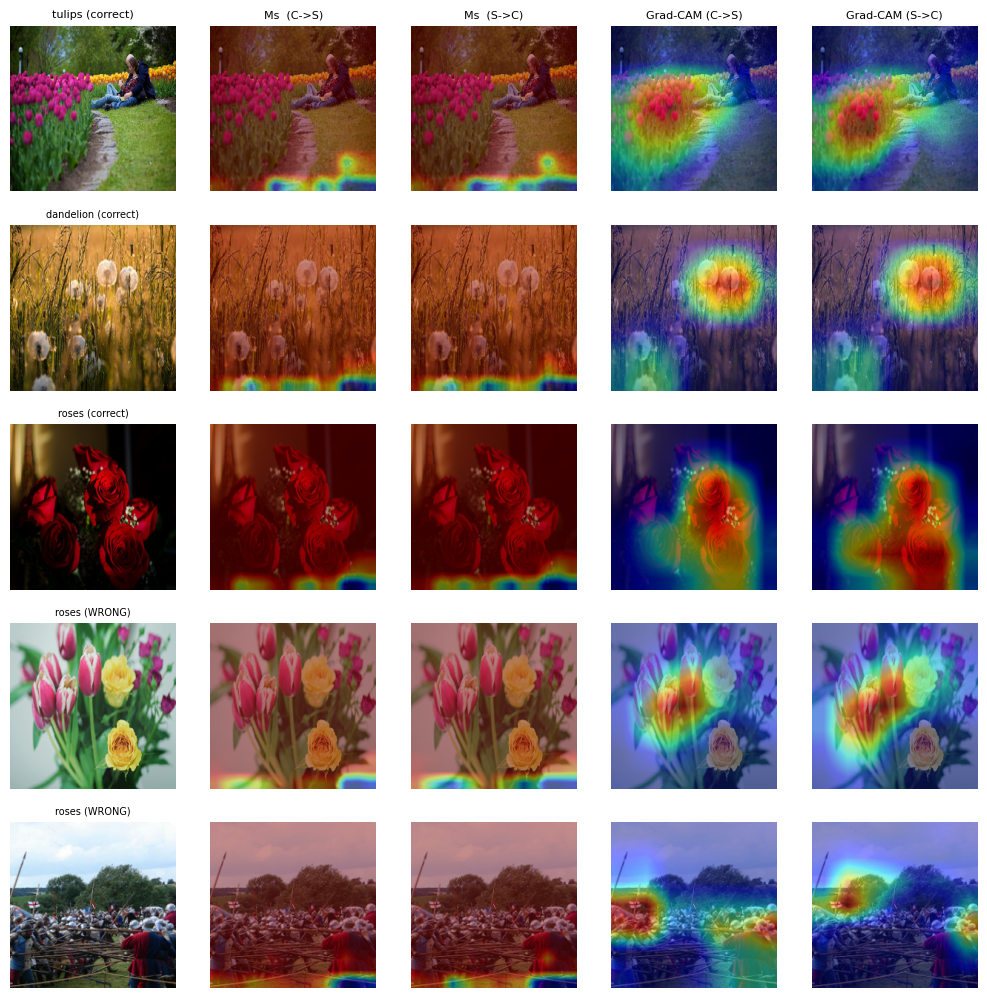
\includegraphics[width=0.8\linewidth]{figs/order_maps.png}
\caption{Experiment 4: spatial attention maps and Grad-CAM for Channel$\to$Spatial (C$\to$S) and Spatial$\to$Channel (S$\to$C) at $P_3$.}
\label{fig:order}
\end{figure}


% ============================================================
\section*{18. Main Experiment 5: Spatial Attention Kernel Size}
% ============================================================

The receptive field used to generate the spatial attention map may influence
the result.

Evaluate:

\[
k\in\{3,5,7\}.
\]

Use the same attention position and training protocol.

\begin{center}

\begin{tabular}{|c|c|c|c|}
\hline

\textbf{Spatial Kernel}
&
\textbf{Accuracy}
&
\textbf{Macro F1}
&
\textbf{Inference Time}
\\
\hline

$3\times3$
& 0.9056
& 0.9056
& 8.01 ms
\\
\hline

$5\times5$
& 0.9310
& 0.9302
& 8.17 ms
\\
\hline

$7\times7$
& 0.9437
& 0.9420
& 8.37 ms
\\
\hline

\end{tabular}

\end{center}

Students should discuss whether a larger spatial kernel provides a useful
increase in contextual information.


\subsection*{Observations: Spatial Kernel Size (Experiment 5)}
\begin{table}[H]
\centering
\caption{Experiment 5 -- spatial kernel size $k$ (Channel$\to$Spatial at $P_3$; $k{=}7$ is A3).}
\scriptsize
\resizebox{\textwidth}{!}{\begin{tabular}{l|cccc|rr|ccc}
\toprule
\textbf{Model} & \textbf{Acc.} & \textbf{Prec.} & \textbf{Recall} & \textbf{Macro F1} & \textbf{Total params} & \textbf{Attn params} & \textbf{Inf.\ ms/img} & \textbf{GFLOPs} & \textbf{Train min}\\
\midrule
E1 C+S, $k{=}3$ & 0.9056 & 0.9044 & 0.9109 & 0.9056 & 23{,}730{,}136 & 132{,}179 & 8.01 & 7.75 & 3.8\\
E2 C+S, $k{=}5$ & 0.9310 & 0.9319 & 0.9303 & 0.9302 & 23{,}730{,}168 & 132{,}211 & 8.17 & 7.75 & 3.8\\
A3 Channel+Spatial & 0.9437 & 0.9469 & 0.9389 & 0.9420 & 23{,}730{,}216 & 132{,}259 & 8.37 & 7.75 & 3.8\\
\bottomrule
\end{tabular}}
\end{table}

Accuracy rises monotonically with the kernel: $3\times3$: 0.9056, $5\times5$: 0.9310, $7\times7$: 0.9437. The $3\times3$ model is essentially the baseline, while $7\times7$ is $3.8$ points better (beyond the noise interval). However, the learned maps do not show a richer use of context for larger kernels (Fig.~\ref{fig:kernel}): the $3\times3$ maps are the most varied (mean 0.787, std 0.224, suppressing the left/bottom border and some textured regions), whereas the $5\times5$ maps are almost saturated (mean 0.972, std 0.059) and the $7\times7$ maps (mean 0.966, std 0.131) are $\approx1$ everywhere except a band along the bottom border. So a larger kernel is associated with higher accuracy, but the maps do not demonstrate that the gain comes from extra spatial context.
\begin{figure}[H]
\centering
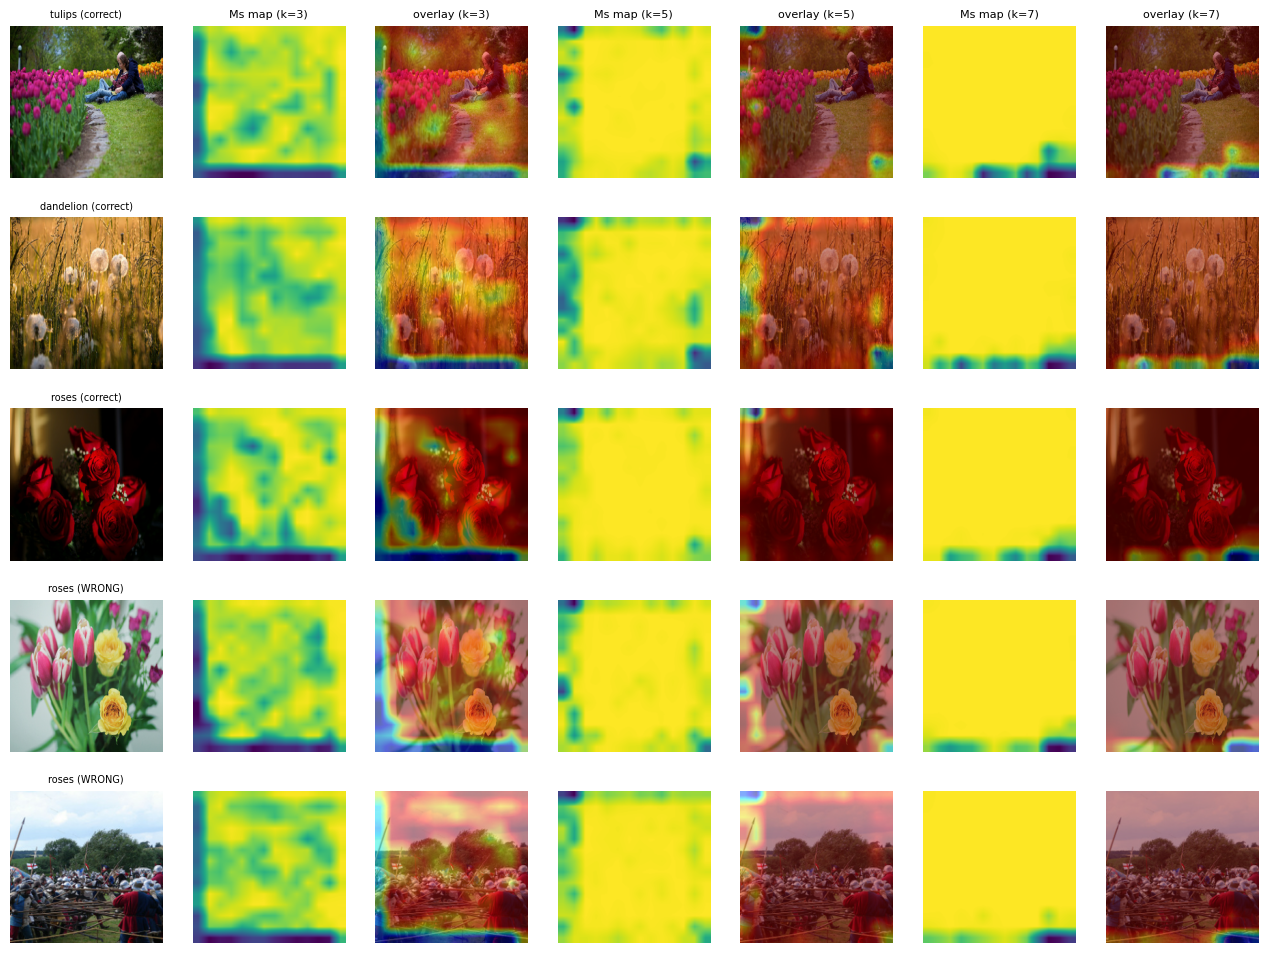
\includegraphics[width=\linewidth]{figs/kernel_maps.png}
\caption{Experiment 5: spatial attention maps and overlays for $k=3,5,7$ at $P_3$.}
\label{fig:kernel}
\end{figure}

\begin{figure}[H]
\centering
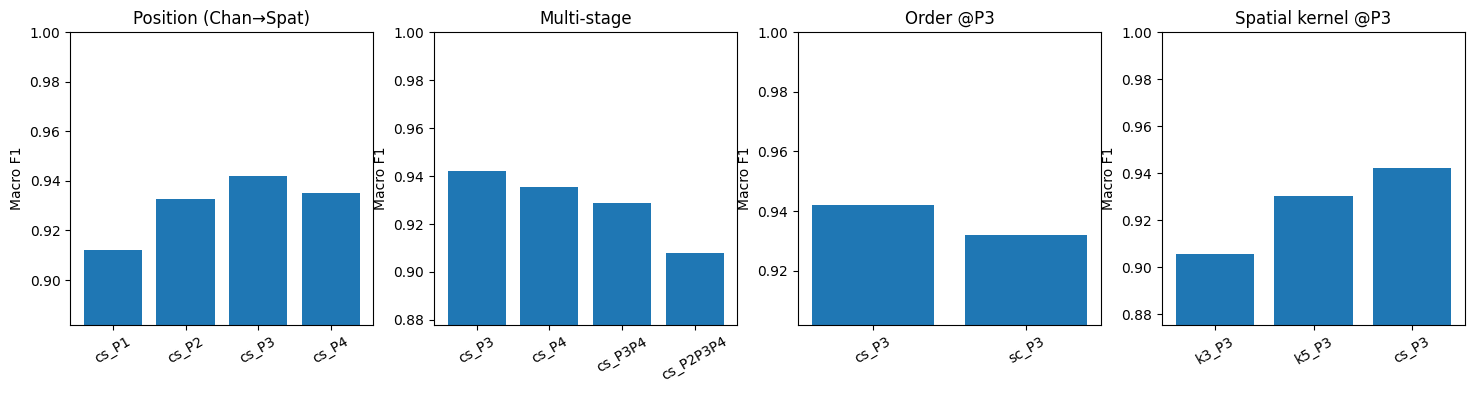
\includegraphics[width=\linewidth]{figs/ablation_groups.png}
\caption{Macro F1 of the position, multi-stage, order and kernel-size ablations.}
\end{figure}



% ============================================================
\section*{19. Additional Task: Comparison of Different Attention Mechanisms}
% ============================================================

As an additional exploration task, students should compare the attention
mechanisms implemented in the laboratory with established attention
approaches.

Students should select at least

\[
\boxed{\text{two additional attention mechanisms}}
\]

from the following:

\begin{itemize}

\item Squeeze-and-Excitation (SE) Attention;

\item Efficient Channel Attention (ECA);

\item Convolutional Block Attention Module (CBAM);

\item Coordinate Attention; and

\item lightweight Self-Attention.

\end{itemize}

The pretrained backbone must remain:

\[
\boxed{\text{ResNet50}}
\]

for all comparisons.

To ensure a fair comparison, additional attention mechanisms should
preferably be inserted at the same position:

\[
\boxed{
P_3=\text{after conv4\_x}
}
\]

unless the student provides a technical justification for using another
location.

% ============================================================
\subsection*{19.1 Suggested Comparison}
% ============================================================

\begin{center}

\resizebox{\textwidth}{!}{
\begin{tabular}{|l|c|c|c|c|c|c|}
\hline

\textbf{Attention}
&
\textbf{Accuracy}
&
\textbf{Precision}
&
\textbf{Recall}
&
\textbf{Macro F1}
&
\textbf{Parameters}
&
\textbf{Inference Time}
\\
\hline

No Attention
& 0.9002
& 0.9116
& 0.9026
& 0.9033
& 23{,}597{,}957
& 8.08 ms
\\
\hline

Channel / SE
& 0.9129
& 0.9159
& 0.9105
& 0.9123
& 23{,}730{,}117
& 8.06 ms
\\
\hline

Spatial Attention
& 0.9419
& 0.9453
& 0.9396
& 0.9419
& 23{,}598{,}056
& 8.17 ms
\\
\hline

ECA
& 0.9238
& 0.9217
& 0.9246
& 0.9222
& 23{,}597{,}962
& 7.77 ms
\\
\hline

CBAM
& 0.9201
& 0.9206
& 0.9203
& 0.9194
& 23{,}730{,}216
& 7.59 ms
\\
\hline

Self-Attention
& 0.9419
& 0.9432
& 0.9400
& 0.9412
& 24{,}908{,}678
& 7.62 ms
\\
\hline

Additional Mechanism (Coordinate Attention)
& 0.9383
& 0.9379
& 0.9373
& 0.9375
& 23{,}698{,}469
& 8.32 ms
\\
\hline

\end{tabular}}
\end{center}


\subsection*{Observations: Performance Results}
The additional-mechanism table of Section 19.1 is filled in above; the main result table of Section 23 is filled in below. The full comparison, including complexity measures, is given here.
\begin{table}[H]
\centering
\caption{Additional-mechanism comparison at $P_3$ (Channel/SE, Spatial, ECA, CBAM, Self-Attention, Coordinate Attention).}
\scriptsize
\resizebox{\textwidth}{!}{\begin{tabular}{l|cccc|rr|ccc}
\toprule
\textbf{Model} & \textbf{Acc.} & \textbf{Prec.} & \textbf{Recall} & \textbf{Macro F1} & \textbf{Total params} & \textbf{Attn params} & \textbf{Inf.\ ms/img} & \textbf{GFLOPs} & \textbf{Train min}\\
\midrule
A0 Baseline & 0.9002 & 0.9116 & 0.9026 & 0.9033 & 23{,}597{,}957 & 0 & 8.08 & 7.75 & 3.6\\
A1 Channel (SE) & 0.9129 & 0.9159 & 0.9105 & 0.9123 & 23{,}730{,}117 & 132{,}160 & 8.06 & 7.75 & 3.7\\
A2 Spatial & 0.9419 & 0.9453 & 0.9396 & 0.9419 & 23{,}598{,}056 & 99 & 8.17 & 7.75 & 3.7\\
F1 ECA & 0.9238 & 0.9217 & 0.9246 & 0.9222 & 23{,}597{,}962 & 5 & 7.77 & 7.75 & 3.8\\
F2 CBAM & 0.9201 & 0.9206 & 0.9203 & 0.9194 & 23{,}730{,}216 & 132{,}259 & 7.59 & 7.75 & 3.8\\
A4 Self-Attention & 0.9419 & 0.9432 & 0.9400 & 0.9412 & 24{,}908{,}678 & 1{,}310{,}721 & 7.62 & 8.35 & 4.1\\
F3 Coordinate Att. & 0.9383 & 0.9379 & 0.9373 & 0.9375 & 23{,}698{,}469 & 100{,}512 & 8.32 & 7.76 & 3.8\\
\bottomrule
\end{tabular}}
\end{table}

\begin{figure}[H]
\centering
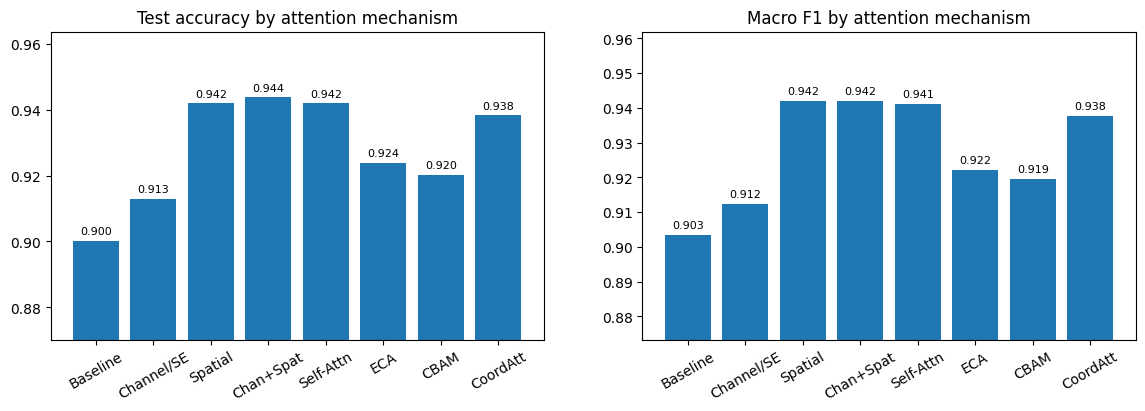
\includegraphics[width=\linewidth]{figs/bar_acc_f1.png}
\caption{Test accuracy and macro F1 by attention mechanism (all at $P_3$).}
\end{figure}

Ranking by accuracy at $P_3$: Channel$\to$Spatial 0.9437 $>$ Spatial = Self-attention 0.9419 $>$ Coordinate 0.9383 $>$ ECA 0.9238 $>$ CBAM 0.9201 $>$ Channel/SE 0.9129 $>$ baseline 0.9002. Macro F1 follows the same ordering (0.942, 0.942, 0.941, 0.938, 0.922, 0.919, 0.912, 0.903). Precision and recall are balanced for every model (differences of at most 0.011), so there is no sign of a model trading one for the other.


% ============================================================
\subsection*{19.2 Questions for Attention-Mechanism Comparison}
% ============================================================

Students should investigate:

\begin{enumerate}

\item How does classification accuracy vary across attention mechanisms?

\item How does macro F1-score vary across attention mechanisms?

\item How many parameters are introduced by each attention module?

\item How does each attention mechanism influence inference time?

\item Does attention improve the convergence behavior?

\item Does attention produce more focused feature localization?

\item Does an increase in attention complexity always improve classification
performance?

\item Does a lightweight attention mechanism provide comparable performance
with a computationally heavier mechanism?

\end{enumerate}

The objective is to understand:

\[
\boxed{
\text{Performance}
+
\text{Complexity}
+
\text{Attention Behaviour}
}
\]

rather than considering only classification accuracy.


\subsection*{Observations: Additional Attention-Mechanism Comparison}
Three additional mechanisms were compared at $P_3$: ECA, CBAM and coordinate attention (SE is the Channel module). Coordinate attention (100{,}512 parameters, 0.9383) is the strongest of them and close to the best models; ECA (5 parameters) improves the baseline by 2.4 points; CBAM (132{,}259 parameters, 0.9201) gives $+2.0$ points and is \emph{worse} than the spatial module alone, which it contains. Answers to the questions of Section 19.2:
\begin{enumerate}
\item \emph{Accuracy:} from 0.9002 (baseline) to 0.9437 (Channel$\to$Spatial).
\item \emph{Macro F1:} from 0.9033 to 0.9420, same ordering.
\item \emph{Parameters:} 5 (ECA), 99 (spatial), 100{,}512 (coordinate), 132{,}160--132{,}259 (SE, Channel$\to$Spatial, CBAM), 1{,}310{,}721 (self-attention), 1{,}442{,}980 (combined).
\item \emph{Inference time:} 7.59--8.37 ms/image with no systematic relation to cost (noise); GFLOPs rise only for self-attention (+0.60).
\item \emph{Convergence:} not accelerated; the train--validation gap and late validation-loss rise are smaller than the baseline's.
\item \emph{Localisation:} only marginal changes (coverage, spread, centre mass differ by about 0.02--0.1).
\item \emph{Complexity vs performance:} more complexity does not always help (combined $<$ Channel$\to$Spatial; $P_2{+}P_3{+}P_4$ $<$ $P_3$; CBAM $<$ spatial).
\item \emph{Lightweight vs heavy:} yes: 99-parameter spatial attention (0.9419) $\approx$ 1.31 M-parameter self-attention (0.9419), and 5-parameter ECA achieves about half of the best gain.
\end{enumerate}


% ============================================================
\section*{20. Transfer-Learning Strategy}
% ============================================================

Use ImageNet pretrained weights.

A recommended training strategy is:

\begin{enumerate}

\item Load ResNet50 with ImageNet pretrained weights.

\item Remove the original ImageNet classification layer.

\item Insert the selected attention module.

\item Add Global Average Pooling.

\item Add Dropout.

\item Add a Dense classification layer containing five output neurons.

\item Initially freeze the pretrained ResNet50 layers.

\item Train the newly introduced attention and classification layers.

\item Unfreeze the final ResNet50 stage or selected final stages.

\item Fine-tune the network using a smaller learning rate.

\end{enumerate}

A suitable initial learning rate for the newly introduced layers is

\[
10^{-3}.
\]

During fine-tuning, a smaller learning rate such as

\[
10^{-5}
\quad\text{to}\quad
10^{-4}
\]

may be used.

The exact values selected by the student should remain identical for all
controlled comparisons.


\subsection*{Observations: Experimental Setup}
All models share the same protocol (Section 34): same split, ImageNet preprocessing (\texttt{resnet50.preprocess\_input}), augmentation (random flip, rotation $\pm5\%$ of a turn, zoom 10\%, translation 10\%, contrast 10\%), seed 42, Adam optimiser, batch size 32, categorical cross-entropy and the same two-phase transfer-learning procedure: \textbf{Phase 1} (5 epochs, learning rate $10^{-3}$): backbone frozen, only attention and head trained; \textbf{Phase 2} (10 epochs, learning rate $10^{-4}$): conv5\_x unfrozen (BatchNorm layers kept frozen). No early stopping or checkpoint selection was used, so all results are \emph{last-epoch} (epoch 15) results. Inference time is the median over three passes on 256 test images (batch 32) on the same GPU; GFLOPs come from the TensorFlow profiler; training time is estimated from the measured median step time scaled to the full protocol.


% ============================================================
\section*{21. Loss Function}
% ============================================================

For the five-class classification problem, use categorical cross-entropy.

For $N$ samples:

\[
\mathcal{L}_{CE}
=
-
\frac{1}{N}
\sum_{i=1}^{N}
\sum_{c=1}^{5}
y_{i,c}
\log
\widehat{y}_{i,c},
\]

where:

\[
y_{i,c}
\]

is the ground-truth label and

\[
\widehat{y}_{i,c}
\]

is the predicted probability.

The same loss formulation must be used for every attention comparison.

% ============================================================
\section*{22. Evaluation Metrics}
% ============================================================

Students must report the following quantitative metrics:

\begin{itemize}

\item classification accuracy;

\item macro precision;

\item macro recall;

\item macro F1-score;

\item number of trainable parameters;

\item total number of parameters; and

\item average inference time per image.

\end{itemize}

For class $c$,

\[
\mathrm{Precision}_c
=
\frac{TP_c}
{TP_c+FP_c},
\]

\[
\mathrm{Recall}_c
=
\frac{TP_c}
{TP_c+FN_c},
\]

and

\[
F1_c
=
2
\frac{
\mathrm{Precision}_c
\mathrm{Recall}_c
}{
\mathrm{Precision}_c+
\mathrm{Recall}_c
}.
\]

Macro F1 is:

\[
\mathrm{Macro\ F1}
=
\frac{1}{C}
\sum_{c=1}^{C}
F1_c,
\]

where

\[
C=5.
\]

% ============================================================
\section*{23. Required Main Result Table}
% ============================================================

Students should summarize the major experiments using the following table.

\begin{center}

\resizebox{\textwidth}{!}{
\begin{tabular}{|l|l|c|c|c|c|c|c|}
\hline

\textbf{Model}
&
\textbf{Position}
&
\textbf{Accuracy}
&
\textbf{Precision}
&
\textbf{Recall}
&
\textbf{F1}
&
\textbf{Parameters}
&
\textbf{Inference Time}
\\
\hline

Baseline
& --
& 0.9002
& 0.9116
& 0.9026
& 0.9033
& 23{,}597{,}957
& 8.08 ms
\\
\hline

Channel Attention
& $P_3$
& 0.9129
& 0.9159
& 0.9105
& 0.9123
& 23{,}730{,}117
& 8.06 ms
\\
\hline

Spatial Attention
& $P_3$
& 0.9419
& 0.9453
& 0.9396
& 0.9419
& 23{,}598{,}056
& 8.17 ms
\\
\hline

Channel+Spatial
& $P_2$
& 0.9328
& 0.9349
& 0.9315
& 0.9326
& 23{,}631{,}368
& 8.03 ms
\\
\hline

Channel+Spatial
& $P_3$
& 0.9437
& 0.9469
& 0.9389
& 0.9420
& 23{,}730{,}216
& 8.37 ms
\\
\hline

Channel+Spatial
& $P_4$
& 0.9365
& 0.9361
& 0.9378
& 0.9351
& 24{,}124{,}520
& 7.87 ms
\\
\hline

Self-Attention
& $P_3$
& 0.9419
& 0.9432
& 0.9400
& 0.9412
& 24{,}908{,}678
& 7.62 ms
\\
\hline

Additional Attention-1 (ECA)
& $P_3$
& 0.9238
& 0.9217
& 0.9246
& 0.9222
& 23{,}597{,}962
& 7.77 ms
\\
\hline

Additional Attention-2 (CBAM)
& $P_3$
& 0.9201
& 0.9206
& 0.9203
& 0.9194
& 23{,}730{,}216
& 7.59 ms
\\
\hline

\end{tabular}}
\end{center}


\subsection*{Observations: Complexity Analysis}
\begin{table}[H]
\centering
\caption{Complexity of all 17 models. GFLOPs from the TensorFlow profiler (one image, multiply-add = 2 FLOPs); training time is the measured median step time scaled to the full 2-phase protocol.}
\scriptsize
\resizebox{\textwidth}{!}{\begin{tabular}{l|rrcccc}
\toprule
\textbf{Model} & \textbf{Total params} & \textbf{Attn params} & \textbf{Param memory (MB)} & \textbf{GFLOPs / image} & \textbf{Est.\ training time (min)} & \textbf{Inference (ms/img)}\\
\midrule
A0 Baseline & 23{,}597{,}957 & 0 & 90 & 7.75 & 3.6 & 8.08\\
A1 Channel (SE) & 23{,}730{,}117 & 132{,}160 & 91 & 7.75 & 3.7 & 8.06\\
A2 Spatial & 23{,}598{,}056 & 99 & 90 & 7.75 & 3.7 & 8.17\\
A3 Channel+Spatial & 23{,}730{,}216 & 132{,}259 & 91 & 7.75 & 3.8 & 8.37\\
A4 Self-Attention & 24{,}908{,}678 & 1{,}310{,}721 & 95 & 8.35 & 4.1 & 7.62\\
A5 Combined (C+S+SA) & 25{,}040{,}937 & 1{,}442{,}980 & 96 & 8.36 & 4.4 & 7.93\\
B1 C+S @ $P_1$ & 23{,}606{,}520 & 8{,}563 & 90 & 7.76 & 5.3 & 8.16\\
B2 C+S @ $P_2$ & 23{,}631{,}368 & 33{,}411 & 90 & 7.75 & 4.5 & 8.03\\
B4 C+S @ $P_4$ & 24{,}124{,}520 & 526{,}563 & 92 & 7.75 & 3.5 & 7.87\\
C1 C+S @ $P_3{+}P_4$ & 24{,}256{,}779 & 658{,}822 & 93 & 7.75 & 3.9 & 7.81\\
C2 C+S @ $P_2{+}P_3{+}P_4$ & 24{,}290{,}190 & 692{,}233 & 93 & 7.76 & 4.7 & 8.41\\
D1 Spatial$\to$Channel & 23{,}730{,}216 & 132{,}259 & 91 & 7.75 & 3.8 & 7.97\\
E1 C+S, $k{=}3$ & 23{,}730{,}136 & 132{,}179 & 91 & 7.75 & 3.8 & 8.01\\
E2 C+S, $k{=}5$ & 23{,}730{,}168 & 132{,}211 & 91 & 7.75 & 3.8 & 8.17\\
F1 ECA & 23{,}597{,}962 & 5 & 90 & 7.75 & 3.8 & 7.77\\
F2 CBAM & 23{,}730{,}216 & 132{,}259 & 91 & 7.75 & 3.8 & 7.59\\
F3 Coordinate Att. & 23{,}698{,}469 & 100{,}512 & 90 & 7.76 & 3.8 & 8.32\\
\bottomrule
\end{tabular}}
\end{table}

\begin{itemize}
\item \textbf{Parameters:} ECA adds 5, spatial attention 99, coordinate attention 100{,}512, Channel/SE, CBAM and Channel$\to$Spatial about 132{,}000 ($+0.56\%$), and self-attention 1{,}310{,}721 ($+5.5\%$). B4 adds 526{,}563 because its channel MLP acts on 2048 channels.
\item \textbf{Computation:} only the self-attention models add noticeable work: 8.35 GFLOPs versus 7.75 for the baseline ($+0.60$, $+7.8\%$). All other modules change the cost by under 0.01 GFLOPs.
\item \textbf{Training time:} the baseline needs about 3.6 min; most single-module models 3.7--3.8 min; self-attention 4.1 min; the combined model 4.4 min; and attention at $P_1$ the most (5.3 min), because the modules operate on the largest feature map.
\item \textbf{Inference time:} all 17 models lie between 7.59 and 8.41 ms/image, and the ordering does \emph{not} follow GFLOPs (e.g.\ self-attention 7.62 ms, CBAM 7.59 ms, baseline 8.08 ms). Differences of $\pm0.5$ ms are therefore measurement noise on a shared Colab GPU, and no latency conclusion can be drawn from them; GFLOPs is the more reliable indicator of cost.
\item \textbf{Memory:} parameter memory is 90 MB for the baseline and 95--96 MB for the self-attention models. Peak-GPU-memory readings were also taken, but the training-memory values increased steadily in the order in which the models were benchmarked (from 1{,}130 MB to 5{,}128 MB), which shows that memory held over from earlier models contaminated them. They are therefore \textbf{not used} here; a clean measurement would require one fresh process per model.
\end{itemize}
\begin{figure}[H]
\centering
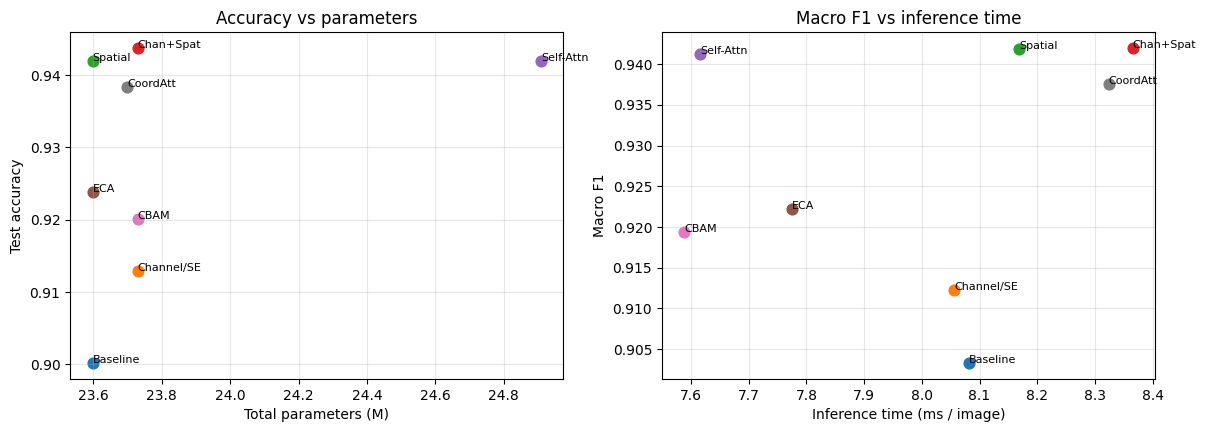
\includegraphics[width=\linewidth]{figs/tradeoffs.png}
\caption{Accuracy versus total parameters (left) and macro F1 versus inference time (right).}
\end{figure}

\textbf{Accuracy--complexity trade-off.} The non-dominated models (fewest parameters for their accuracy) are the baseline, Spatial (A2), Channel$\to$Spatial (A3) and ECA. \textbf{F1--time trade-off:} Spatial, Channel$\to$Spatial, Self-attention and CBAM are non-dominated, but given the timing noise this set should not be over-interpreted. A rank correlation of $+0.39$ between attention parameters and accuracy over the nine $P_3$ models shows at best a weak link: the largest module (combined, 1.44 M) is not the most accurate, whereas the 99-parameter spatial module is among the best.


% ============================================================
\section*{24. Graphical Performance Analysis}
% ============================================================

Students should not present only numerical tables.

Appropriate graphs must be generated to analyze model behavior.

At least three of the following graphical comparisons should be included in
the laboratory report.

% ============================================================
\subsection*{24.1 Training and Validation Accuracy}
% ============================================================

Plot

\[
\text{Epoch}
\quad\text{versus}\quad
\text{Accuracy}
\]

for:

\begin{itemize}

\item baseline ResNet50; and

\item selected attention models.

\end{itemize}

Both training and validation accuracy should be shown.

Students should comment on whether attention:

\begin{itemize}

\item accelerates convergence;

\item produces smoother learning;

\item reduces the train--validation gap;

\item leads to overfitting; or

\item causes unstable training.

\end{itemize}

% ============================================================
\subsection*{24.2 Training and Validation Loss}
% ============================================================

Plot

\[
\text{Epoch}
\quad\text{versus}\quad
\mathcal{L}_{CE}.
\]

The graph should include training and validation loss.

Students should compare the convergence behavior of the baseline and
attention models.


\subsection*{Observations: Training and Validation Graphs}
\begin{figure}[H]
\centering
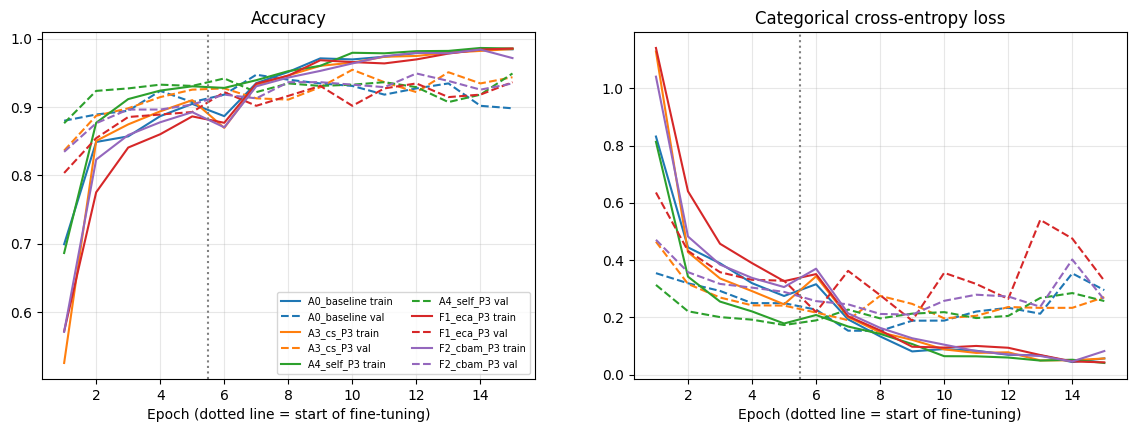
\includegraphics[width=\linewidth]{figs/training_curves.png}
\caption{Training (solid) and validation (dashed) accuracy and cross-entropy loss; dotted line = start of fine-tuning.}
\end{figure}

\begin{figure}[H]
\centering
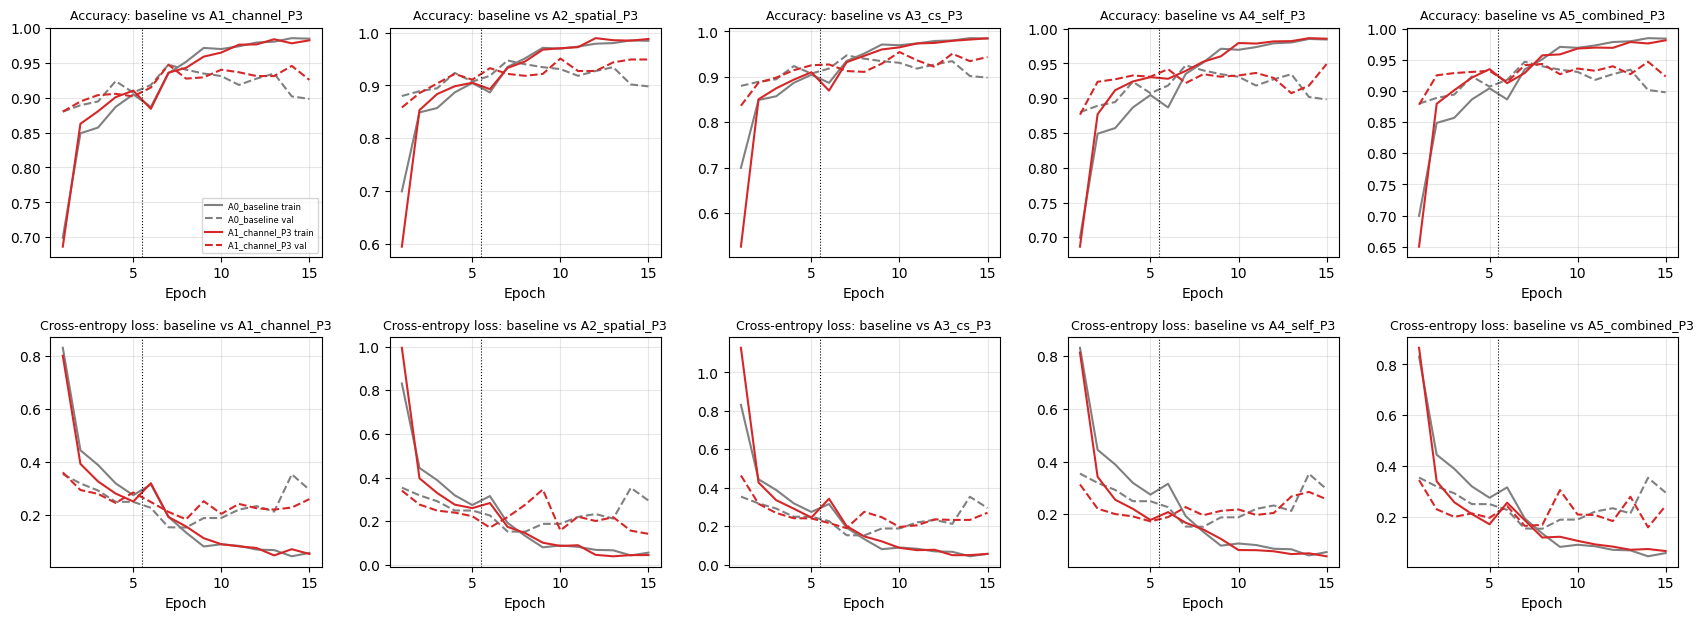
\includegraphics[width=\linewidth]{figs/curves_each.png}
\caption{Baseline (grey) versus each attention-type model (red): accuracy (top) and loss (bottom).}
\end{figure}

\begin{table}[H]
\centering
\caption{Observation sheet (Section 38): last-epoch training/validation metrics (epoch 15) and test accuracy for all 17 runs. Training metrics are measured with augmentation and dropout active.}
\scriptsize
\resizebox{\textwidth}{!}{\begin{tabular}{l|cccccccr}
\toprule
\textbf{Model} & \textbf{Train acc} & \textbf{Val acc} & \textbf{Test acc} & \textbf{Train loss} & \textbf{Val loss} & \textbf{Train$-$Val acc} & \textbf{Best-val epoch} & \textbf{Trainable (final)}\\
\midrule
A0 Baseline & 0.9844 & 0.8982 & 0.9002 & 0.0567 & 0.2952 & 0.0862 & 7 & 14{,}963{,}717\\
A1 Channel (SE) & 0.9821 & 0.9255 & 0.9129 & 0.0530 & 0.2599 & 0.0566 & 7 & 15{,}095{,}877\\
A2 Spatial & 0.9879 & 0.9491 & 0.9419 & 0.0456 & 0.1429 & 0.0388 & 10 & 14{,}963{,}816\\
A3 Channel+Spatial & 0.9848 & 0.9436 & 0.9437 & 0.0565 & 0.2705 & 0.0412 & 10 & 15{,}095{,}976\\
A4 Self-Attention & 0.9856 & 0.9491 & 0.9419 & 0.0408 & 0.2570 & 0.0365 & 15 & 16{,}274{,}438\\
A5 Combined (C+S+SA) & 0.9817 & 0.9236 & 0.9274 & 0.0646 & 0.2431 & 0.0581 & 14 & 16{,}406{,}697\\
B1 C+S @ $P_1$ & 0.9910 & 0.8927 & 0.9129 & 0.0346 & 0.3159 & 0.0983 & 14 & 14{,}972{,}280\\
B2 C+S @ $P_2$ & 0.9708 & 0.9255 & 0.9328 & 0.0814 & 0.1996 & 0.0454 & 7 & 14{,}997{,}128\\
B4 C+S @ $P_4$ & 0.9825 & 0.9309 & 0.9365 & 0.0526 & 0.2445 & 0.0516 & 14 & 15{,}490{,}280\\
C1 C+S @ $P_3{+}P_4$ & 0.9868 & 0.9382 & 0.9292 & 0.0364 & 0.1955 & 0.0486 & 15 & 15{,}622{,}539\\
C2 C+S @ $P_2{+}P_3{+}P_4$ & 0.9879 & 0.9055 & 0.9074 & 0.0409 & 0.3025 & 0.0825 & 14 & 15{,}655{,}950\\
D1 Spatial$\to$Channel & 0.9661 & 0.9364 & 0.9328 & 0.1015 & 0.2357 & 0.0298 & 14 & 15{,}095{,}976\\
E1 C+S, $k{=}3$ & 0.9700 & 0.9236 & 0.9056 & 0.0771 & 0.2316 & 0.0464 & 13 & 15{,}095{,}896\\
E2 C+S, $k{=}5$ & 0.9755 & 0.9400 & 0.9310 & 0.0846 & 0.3243 & 0.0355 & 10 & 15{,}095{,}928\\
F1 ECA & 0.9856 & 0.9364 & 0.9238 & 0.0429 & 0.3277 & 0.0492 & 15 & 14{,}963{,}722\\
F2 CBAM & 0.9716 & 0.9345 & 0.9201 & 0.0824 & 0.2613 & 0.0370 & 12 & 15{,}095{,}976\\
F3 Coordinate Att. & 0.9782 & 0.9509 & 0.9383 & 0.0695 & 0.2610 & 0.0273 & 14 & 15{,}064{,}165\\
\bottomrule
\end{tabular}}
\end{table}

Observations (Section 24.1/24.2):
\begin{itemize}
\item \textbf{Convergence speed:} no consistent acceleration. The first epoch with validation accuracy $\ge0.88$ is epoch 2 for the baseline and for A1--A5; only C1 reaches it in epoch 1, while B1 needs 6 epochs, E1 4 and ECA, CBAM, Coordinate and E2 3.
\item \textbf{Train--validation gap:} the baseline's gap (0.0862) is larger than that of every attention model except B1 (0.0983); the others range from 0.027 to 0.083, e.g.\ A2 0.039, A3 0.041, A4 0.037, Coordinate 0.027. Part of this is because the baseline's validation accuracy decays late in training (best at epoch 7, 0.8982 at epoch 15).
\item \textbf{Overfitting:} the baseline's validation loss rises from its minimum (epoch 8) by 0.14; A2's validation loss is still decreasing at epoch 15 (rise 0.000); by train--validation gap, B1 (0.0983) and the three-stage model C2 (0.0825) overfit most among the attention models, and ECA and E2 show validation-loss rises (0.139, 0.133) similar to the baseline's.
\item \textbf{Smoothness / instability:} no consistent effect. Epoch-to-epoch validation-accuracy roughness is 0.0130 for the baseline, lower for A1, CBAM and D1 and higher for most others (e.g.\ A3 0.0170, ECA 0.0194, $k{=}3$ 0.0368); B4, A4, A5, C1 and E2 have more validation-loss increases (6--7) than the baseline (5). All curves jump when fine-tuning starts (epoch 6).
\end{itemize}


% ============================================================
\subsection*{24.3 Attention Mechanism versus Accuracy}
% ============================================================

Generate a bar graph:

\[
x=
\text{Attention Mechanism}
\]

and

\[
y=
\text{Classification Accuracy}.
\]

Possible entries are:

\begin{center}

Baseline,
Channel,
Spatial,
Channel+Spatial,
Self-Attention,
SE,
ECA,
CBAM.

\end{center}

% ============================================================
\subsection*{24.4 Attention Mechanism versus Macro F1}
% ============================================================

Similarly, plot:

\[
x=
\text{Attention Mechanism}
\]

and

\[
y=
\text{Macro F1-score}.
\]

This comparison is useful when the class-wise performance is not uniform.

% ============================================================
\subsection*{24.5 Accuracy versus Model Parameters}
% ============================================================

Create a scatter plot using:

\[
x=
\text{Total Model Parameters}
\]

and

\[
y=
\text{Test Accuracy}.
\]

Each point should represent one attention mechanism.

This allows the student to study the

\[
\boxed{
\text{Accuracy--Complexity Trade-off}
}
\]

instead of evaluating accuracy independently.

% ============================================================
\subsection*{24.6 Macro F1 versus Inference Time}
% ============================================================

Plot:

\[
x=
\text{Inference Time per Image}
\]

and

\[
y=
\text{Macro F1-score}.
\]

Students should analyze whether additional computational cost produces a
meaningful increase in classification performance.

% ============================================================
\section*{25. Confusion Matrix Analysis}
% ============================================================

Generate a confusion matrix for:

\begin{enumerate}

\item baseline ResNet50; and

\item the selected attention-based ResNet50.

\end{enumerate}

The confusion matrix should contain all five flower classes.

Students should analyze:

\begin{itemize}

\item which classes are most accurately classified;

\item which classes are frequently confused;

\item which class benefits most from attention;

\item whether attention reduces a particular type of confusion; and

\item whether the improved overall accuracy is distributed across classes.

\end{itemize}


\subsection*{Observations: Confusion Matrix Analysis}
\begin{figure}[H]
\centering
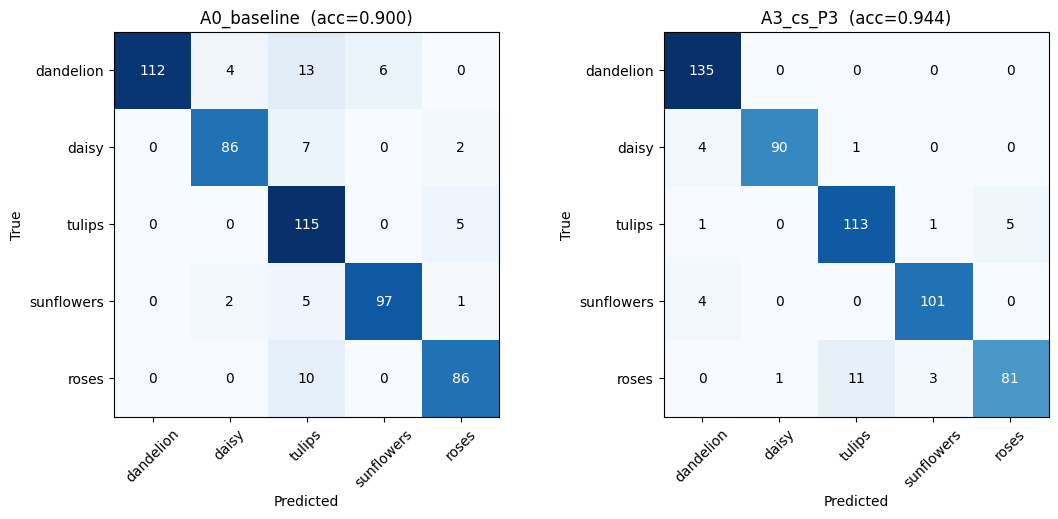
\includegraphics[width=0.85\linewidth]{figs/confusion_matrices.png}
\caption{Confusion matrices (551 test images): baseline A0 and selected model A3.}
\end{figure}

\begin{table}[H]
\centering
\caption{Per-class comparison of the baseline (A0) and the selected model (A3, Channel$\to$Spatial at $P_3$).}
\scriptsize
\resizebox{\textwidth}{!}{\begin{tabular}{l|ccccccc}
\toprule
\textbf{Class} & \textbf{Test images} & \textbf{Recall A0} & \textbf{Recall A3} & \textbf{$\Delta$ recall} & \textbf{F1 A0} & \textbf{F1 A3} & \textbf{$\Delta$ F1}\\
\midrule
dandelion & 135 & 0.830 & 1.000 & $+0.170$ & 0.907 & 0.968 & $+0.061$\\
daisy & 95 & 0.905 & 0.947 & $+0.042$ & 0.920 & 0.968 & $+0.048$\\
tulips & 120 & 0.958 & 0.942 & $-0.017$ & 0.852 & 0.922 & $+0.071$\\
sunflowers & 105 & 0.924 & 0.962 & $+0.038$ & 0.933 & 0.962 & $+0.029$\\
roses & 96 & 0.896 & 0.844 & $-0.052$ & 0.905 & 0.890 & $-0.015$\\
\bottomrule
\end{tabular}}
\end{table}

\begin{itemize}
\item \textbf{Most accurately classified:} tulips for the baseline (recall 0.958), dandelion for A3 (all 135 correct).
\item \textbf{Frequent confusions:} the baseline mainly predicts \emph{tulips} for other classes (dandelion$\to$tulips 13, roses$\to$tulips 10, daisy$\to$tulips 7) and dandelion$\to$sunflowers 6.
\item \textbf{What attention reduced:} dandelion$\to$tulips fell from 13 to 0, daisy$\to$tulips from 7 to 1 and dandelion$\to$sunflowers from 6 to 0. Total errors fell from 55 to 31.
\item \textbf{What it did not:} roses$\to$tulips stayed (10 vs 11) and roses recall fell from 0.896 to 0.844. New, small confusions appeared (sunflowers$\to$dandelion 4, daisy$\to$dandelion 4).
\item \textbf{Which class benefits most:} tulips (F1 $+0.071$ for A3) and dandelion (recall $+0.170$); averaged over all 16 attention variants tulips gains most, whereas roses gains least or loses (Fig.~\ref{fig:pcf1}).
\item \textbf{Distribution:} four of five classes improve in F1 with A3, so the gain is broad, but roses does not benefit.
\end{itemize}
\begin{figure}[H]
\centering
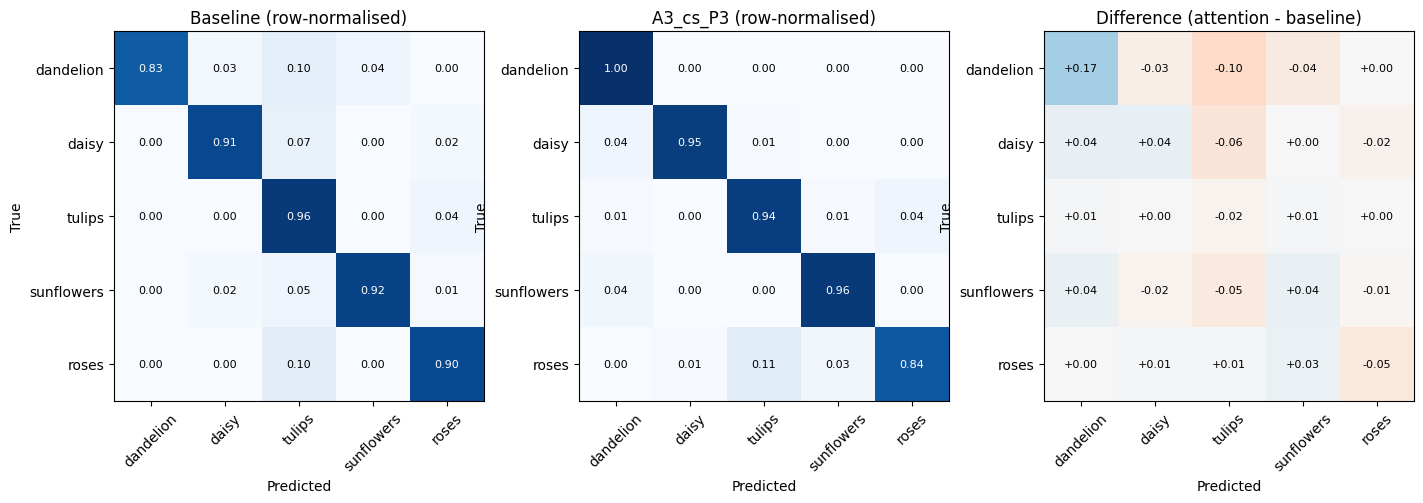
\includegraphics[width=\linewidth]{figs/confusion_norm_diff.png}
\caption{Row-normalised confusion matrices and their difference (attention $-$ baseline).}
\end{figure}

\begin{figure}[H]
\centering
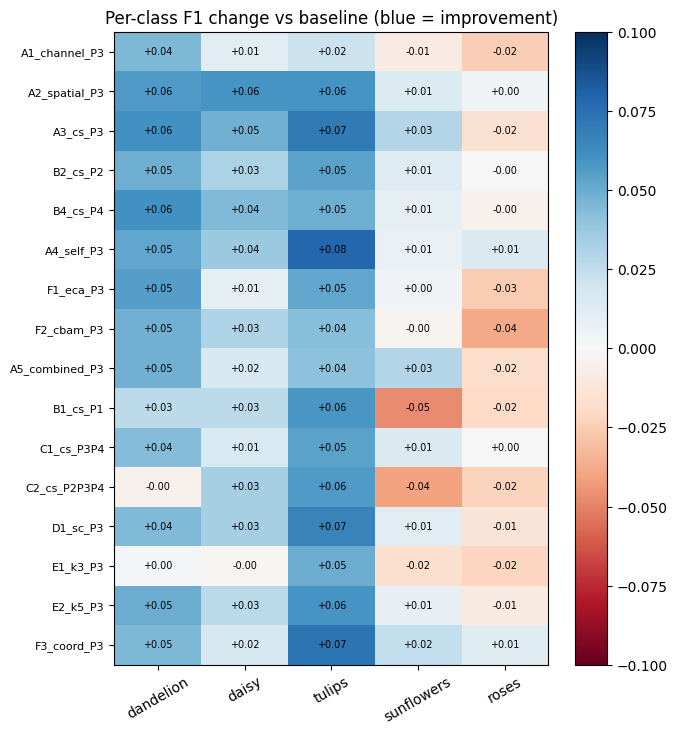
\includegraphics[width=0.55\linewidth]{figs/per_class_f1_change.png}
\caption{Per-class F1 change relative to the baseline for all attention variants.}
\label{fig:pcf1}
\end{figure}



% ============================================================
\section*{26. Qualitative Analysis of Attention}
% ============================================================

Quantitative classification performance does not directly explain where the
network obtains evidence for its prediction.

Students must therefore perform qualitative analysis.

The visual analysis should include:

\begin{itemize}

\item internal attention maps;

\item attention overlays;

\item intermediate feature maps; and

\item Grad-CAM explanations.

\end{itemize}

Students should preferably use the same input image when comparing different
models.


\subsection*{Observations: Test Images and Feature Maps}
Five fixed test images were used for all qualitative figures: three correctly classified (tulips, dandelion, roses) and two roses images that the selected model A3 misclassified.
\begin{figure}[H]
\centering
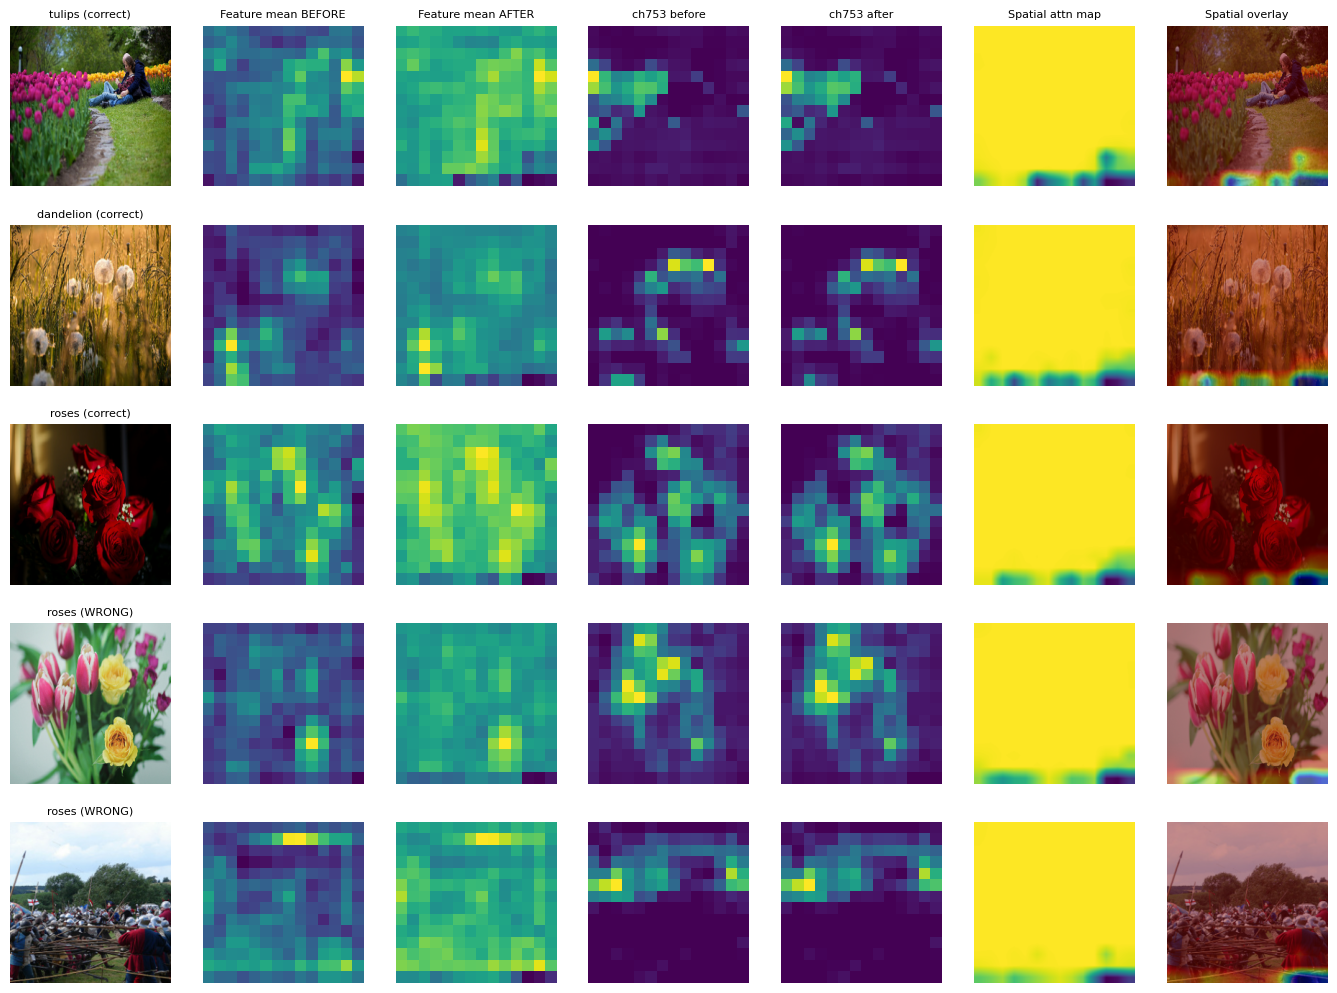
\includegraphics[width=\linewidth]{figs/features_spatial.png}
\caption{Feature maps before/after the $P_3$ Channel$\to$Spatial module, selected channel before/after, spatial attention map and overlay for the five test images.}
\label{fig:feat}
\end{figure}


% ============================================================
\section*{27. Grad-CAM Visualization}
% ============================================================

Gradient-weighted Class Activation Mapping (Grad-CAM) provides a
class-specific visualization of the regions contributing to a prediction.

Let

\[
A^k
\]

represent feature map $k$ from a selected convolutional layer.

For class score $y^c$, the importance coefficient is:

\[
\alpha_k^c
=
\frac{1}{HW}
\sum_i
\sum_j
\frac{\partial y^c}
{\partial A_{ij}^k}.
\]

The Grad-CAM map is:

\[
L_{\mathrm{Grad-CAM}}^c
=
\operatorname{ReLU}
\left(
\sum_k
\alpha_k^c A^k
\right).
\]

The map should be resized to the original image resolution and overlaid on
the input.

Students should compare:

\[
\boxed{
\text{Input}
\;|\;
\text{Baseline Grad-CAM}
\;|\;
\text{Attention Model Grad-CAM}
}
\]

for the same image.

% ============================================================
\subsection*{27.1 Grad-CAM Interpretation}
% ============================================================

Students should qualitatively determine whether the attention model:

\begin{itemize}

\item focuses more strongly on the flower;

\item suppresses irrelevant background regions;

\item concentrates on petals;

\item concentrates on the central flower structure;

\item attends to discriminative edges;

\item distributes activation across the entire flower;

\item incorrectly focuses on leaves;

\item incorrectly focuses on background objects; or

\item changes its focus for an incorrect prediction.

\end{itemize}

Students should avoid unsupported statements such as:

\begin{quote}
``The Grad-CAM of Model A is better.''
\end{quote}

Instead, the observation should describe visible evidence.

For example:

\begin{quote}
The baseline network activates both the flower and surrounding leaves,
whereas the attention-based model produces stronger activation over the petal
region and weaker activation over the background.
\end{quote}


\subsection*{Observations: Grad-CAM Analysis}
\begin{figure}[H]
\centering
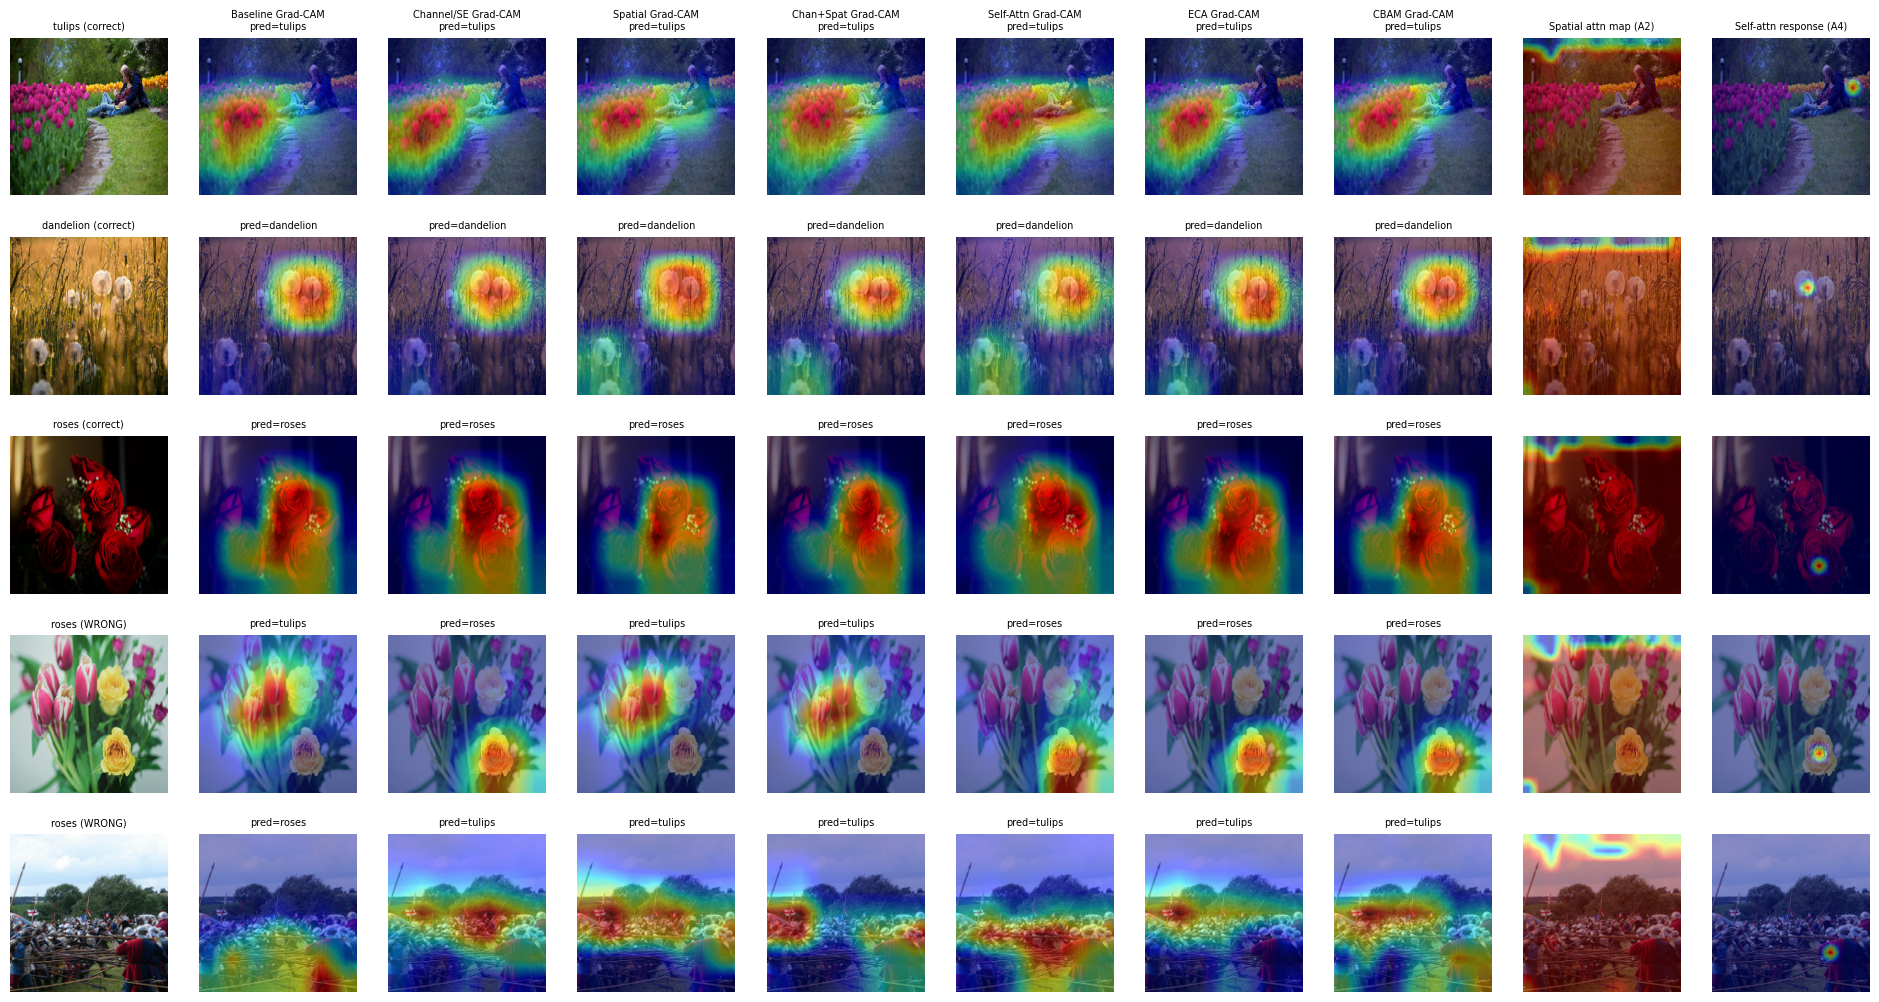
\includegraphics[width=\linewidth]{figs/gradcam_comparison.png}
\caption{Grad-CAM of baseline, Channel/SE, Spatial, Channel+Spatial, Self-attention, ECA and CBAM models, plus the spatial map of A2 and the self-attention response of A4, for the same five images.}
\end{figure}

Grad-CAM (post-hoc, computed from gradients of the class score at the last convolutional stage) differs fundamentally from the internal attention maps of Sections 28 and 29, which are computed inside the forward pass. Visible evidence for the five images:
\begin{itemize}
\item \textbf{Tulips (correct):} all models focus on the dense pink tulip bed on the left; the Channel$\to$Spatial and self-attention models spread somewhat more activation toward the path and the seated people.
\item \textbf{Dandelion (correct):} every model centres on the two seed heads; spatial, Channel$\to$Spatial and self-attention add a weaker secondary blob on the lower-left dandelion.
\item \textbf{Roses (correct):} all models concentrate on the central rose cluster; the maps differ only slightly in compactness.
\item \textbf{Roses, wrong for A3 (bouquet of pink tulips and yellow roses):} the baseline, spatial and Channel$\to$Spatial models predict \emph{tulips} with activation on the pink tulips, whereas the channel, ECA, CBAM and self-attention models predict \emph{roses} with activation on the lower yellow rose. The prediction follows the region the model attends to.
\item \textbf{Roses, wrong for A3 (crowd scene without a prominent flower):} the baseline predicts roses with activation on the red clothing at the lower right, whereas all attention models predict tulips with a horizontal band of activation across the crowd/ground, i.e.\ evidence is scene-level and not on a flower; this image is atypical for the class.
\end{itemize}
Observations from five images are illustrative only; Section 30 checks them on 100 images.


% ============================================================
\section*{28. Internal Attention Maps}
% ============================================================

An important objective of this experiment is to distinguish between:

\[
\boxed{\text{Internal Attention}}
\]

and

\[
\boxed{\text{Post-hoc Explanation}}
\]

because they are not the same.

An attention module directly computes weights during the forward pass.

Grad-CAM, in contrast, is generated after prediction using gradients.

% ============================================================
\subsection*{28.1 Channel-Attention Visualization}
% ============================================================

For channel attention:

\[
M_c(F)
=
[m_1,m_2,\ldots,m_C].
\]

Students should visualize the learned channel importance values using a bar
graph.

Instead of displaying every channel when $C$ is large, the student may show
the top-$K$ channels.

Recommended values are:

\[
K=10
\]

or

\[
K=20.
\]

Students should comment on whether:

\begin{itemize}

\item a small number of channels receive strong weights;

\item many channels contribute similarly; or

\item channel weighting changes substantially for different input images.

\end{itemize}


\subsection*{Observations: Channel Attention}
\begin{figure}[H]
\centering
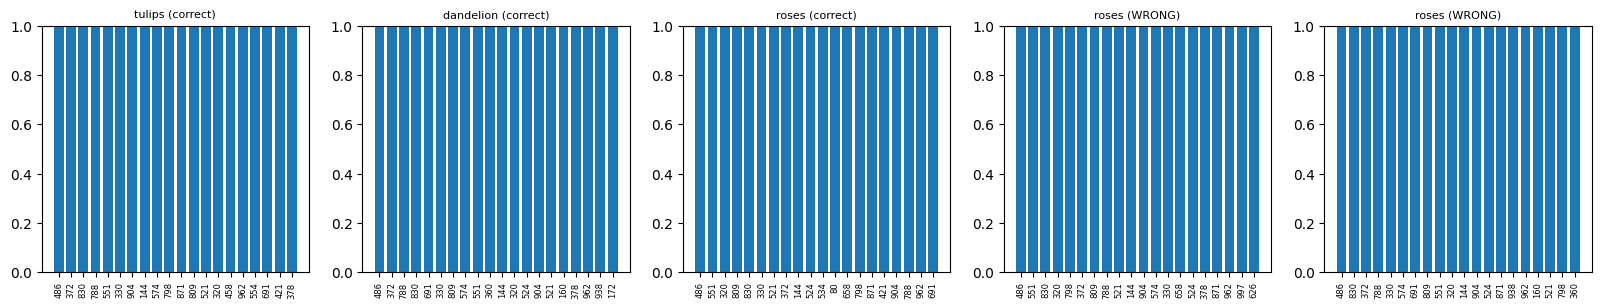
\includegraphics[width=\linewidth]{figs/channel_weights.png}
\caption{Top-20 channel-attention weights (channel gate of A3 at $P_3$) for the five test images.}
\end{figure}

For the channel gate of the selected model A3 (Channel$\to$Spatial at $P_3$) the weights are strongly bimodal (mean 0.583, standard deviation 0.417 over the 1024 channels); the top-20 channels of every image are all saturated at $\approx1.0$, and the weight vectors of different images are almost identical (mean pairwise correlation \textbf{0.997}). Thus a large group of channels receives strong weights, many others are suppressed, and the channel weighting hardly changes with the input: in practice it acts as a learned, nearly static channel selection rather than an image-adaptive one. (For the same reason the ``top-$K$'' ranking is unstable: the overlap of the top-20 channels between the two attention orders is only 3--4 of 20, but many channels tie at $\approx1$, so this overlap is not informative.) The feature maps before and after attention look alike for single channels (e.g.\ channel 753) while the mean feature map after attention is smoother, with more activation on background regions.

% ============================================================
\subsection*{28.2 Spatial-Attention Visualization}
% ============================================================

For spatial attention:

\[
M_s(F)
\in
\mathbb{R}^{H\times W}.
\]

Resize the attention map to:

\[
224\times224
\]

and overlay it on the input image.

Display:

\[
\boxed{
\text{Input}
\;|\;
\text{Spatial Attention Map}
\;|\;
\text{Attention Overlay}
}
\]

Students should identify the image regions receiving high attention values.


\subsection*{Observations: Spatial Attention}
In Fig.~\ref{fig:feat} and Fig.~\ref{fig:pos} the spatial maps are $\approx1$ (full pass-through) over most of the image; the low values appear \textbf{mainly along the bottom border and in a corner}, not on the flower or the background clutter. This pattern is probably linked to zero padding of the $7\times7$ convolution at the feature-map border, so the spatial gate acts mostly as a border-suppression (and re-scaling) mechanism rather than as a flower detector. The strong accuracy gain of A2/A3 should be read in this light: it is real in the test numbers, but the maps do not show semantic foreground selection, and the single-run protocol cannot separate the effect of the gate from other effects (for example, regularisation of the fine-tuned conv5\_x stage).

% ============================================================
\subsection*{28.3 Self-Attention Visualization}
% ============================================================

For self-attention, students may visualize one of the following:

\begin{itemize}

\item attention associated with a selected query location;

\item mean attention across query positions;

\item maximum attention across query positions; or

\item an aggregated spatial self-attention response.

\end{itemize}

The visualization should be reshaped into a spatial form and, when
appropriate, resized to the image resolution.

Students should analyze how distant regions interact within the feature map.


\subsection*{Observations: Self-Attention}
\begin{figure}[H]
\centering
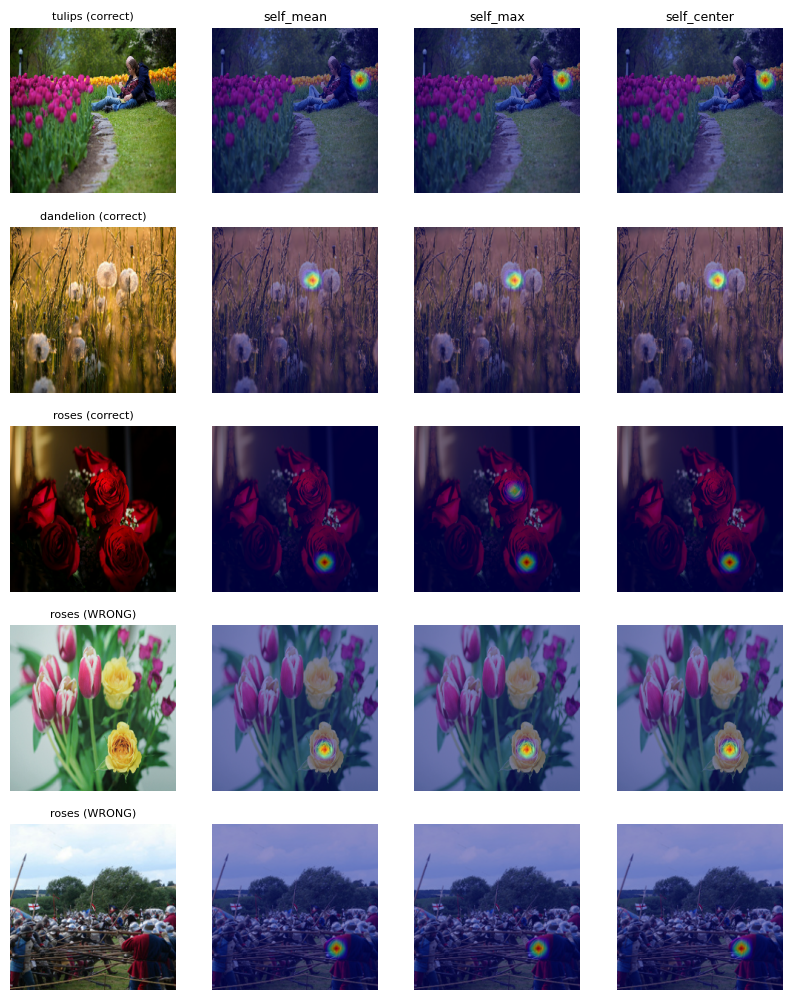
\includegraphics[width=0.7\linewidth]{figs/self_attention.png}
\caption{Self-attention responses (mean over queries, maximum over queries, centre query) at $P_3$.}
\end{figure}

The learned residual scale reached only $\gamma=0.059$, so the self-attention branch contributes a small correction. The mean-, maximum- and centre-query responses are almost identical and show a \textbf{single compact hot spot} per image (on a dandelion head, on a rose, on the yellow rose in the first wrong image and on the red clothing in the crowd image, but near the person rather than the tulips in the first image). Hence most query positions attend to the same few key positions (a ``hub'' pattern): distant regions interact through one dominant location rather than through broad pairwise relations. The $N\times N$ matrix has 38{,}416 entries per image at $P_3$.
\begin{table}[H]
\centering
\caption{Growth of the self-attention matrix with resolution ($d=C/8$, fp32, one head).}
\scriptsize
\resizebox{\textwidth}{!}{\begin{tabular}{l|cccccc}
\toprule
\textbf{Position} & \textbf{Feature map} & \textbf{$N=HW$} & \textbf{$N\times N$ entries} & \textbf{Matrix size / image (MB)} & \textbf{Self-attn params} & \textbf{Self-attn MACs (M)}\\
\midrule
$P_1$ & $56\times56\times256$ & 3136 & 9{,}834{,}496 & 37.52 & 81{,}921 & 3089.2\\
$P_2$ & $28\times28\times512$ & 784 & 614{,}656 & 2.34 & 327{,}681 & 610.9\\
$P_3$ & $14\times14\times1024$ & 196 & 38{,}416 & 0.15 & 1{,}310{,}721 & 301.2\\
$P_4$ & $7\times7\times2048$ & 49 & 2{,}401 & 0.01 & 5{,}242{,}881 & 262.4\\
\bottomrule
\end{tabular}}
\end{table}


% ============================================================
\section*{29. Attention Position Visualization}
% ============================================================

Use the same test image to visualize spatial attention at different ResNet50
stages.

Generate:

\[
M_s^{P_2},
\qquad
M_s^{P_3},
\qquad
M_s^{P_4}.
\]

Display the maps as:

\[
\boxed{
\text{Input}
\;|\;
M_s^{P_2}
\;|\;
M_s^{P_3}
\;|\;
M_s^{P_4}
}
\]

The objective is to visually study how attention changes as feature
representations become deeper.

Possible observations may include:

\begin{itemize}

\item $P_2$ responding strongly to edges, colors, textures, and fine
structures;

\item $P_3$ responding to flower parts and intermediate object structures;

\item $P_4$ responding to larger semantic flower regions.

\end{itemize}

These observations must be based on the student's experimental
visualizations.


\subsection*{Observations: Attention at $P_2$, $P_3$ and $P_4$}
\begin{figure}[H]
\centering
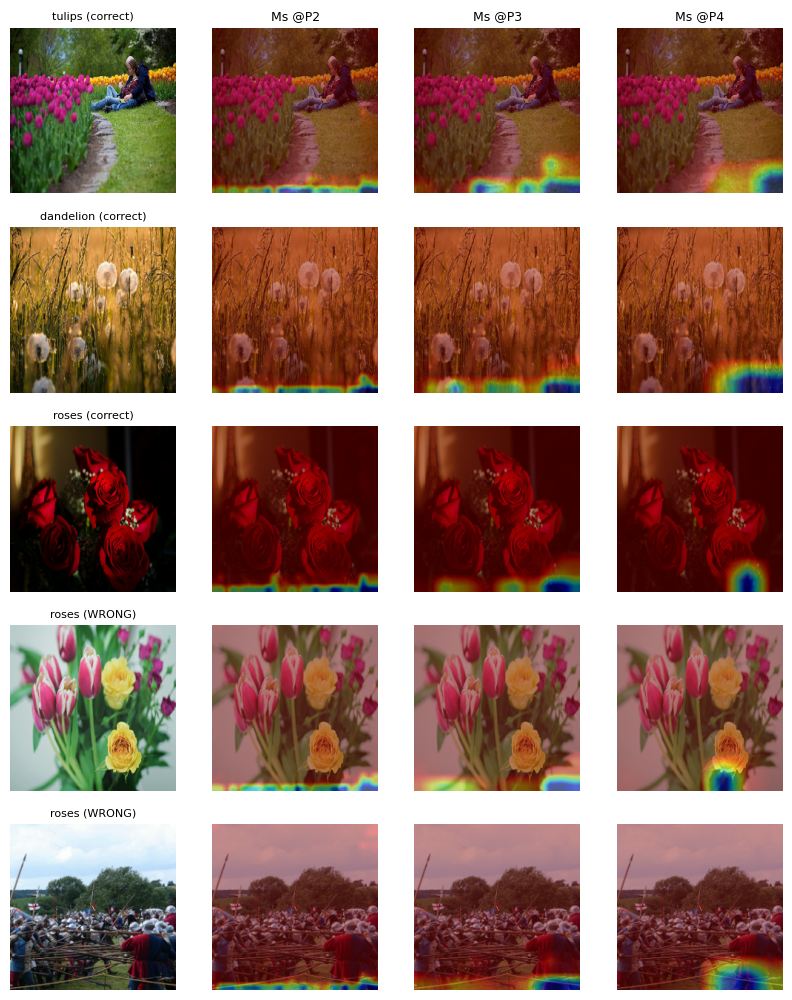
\includegraphics[width=0.7\linewidth]{figs/attention_P2_P3_P4.png}
\caption{Spatial attention maps $M_s^{P_2}$, $M_s^{P_3}$, $M_s^{P_4}$ for the same five images.}
\label{fig:pos}
\end{figure}

The three maps (from separately trained models) differ mainly in the size and place of the low-valued region: a thin band along the bottom edge at $P_2$ ($28\times28$), a wider band in the lower right at $P_3$, and a compact blob in the lower right at $P_4$ ($7\times7$), consistent with the coarser feature grid. The expectation ``$P_2$ responds to edges and textures, $P_4$ to larger semantic regions'' \textbf{is not confirmed} by these figures, because in all three maps the flower regions are left at $\approx1$. When all stages carry attention in the same network (C2, Fig.~\ref{fig:ms}), the maps change again (vertical low-valued strips at $P_3$ and $P_4$), which shows that the maps depend on what the other modules do.
\begin{figure}[H]
\centering
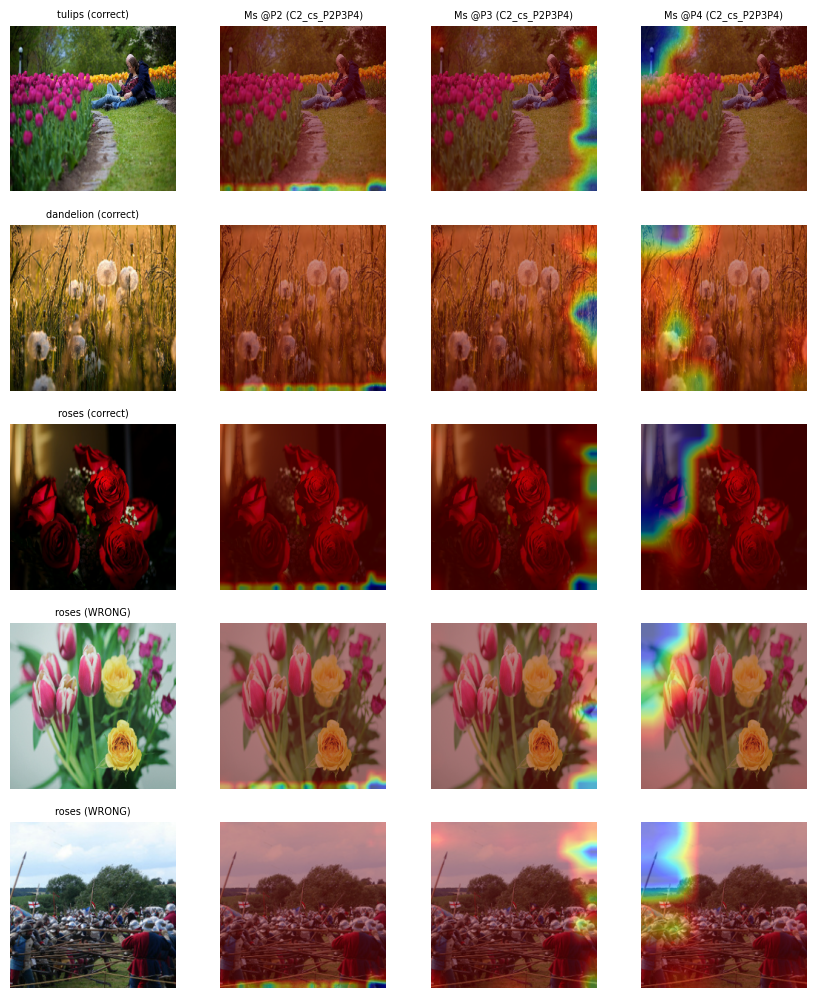
\includegraphics[width=0.6\linewidth]{figs/multistage_C2.png}
\caption{Spatial maps of the three-stage model C2 ($P_2{+}P_3{+}P_4$).}
\label{fig:ms}
\end{figure}



% ============================================================
\section*{30. Qualitative Comparison Across Attention Mechanisms}
% ============================================================

Select at least:

\[
\boxed{
3\text{ correctly classified images}
}
\]

and

\[
\boxed{
2\text{ incorrectly classified images}.
}
\]

For every selected image, compare the behavior of multiple models.

A recommended arrangement is:

\[
\boxed{
\begin{array}{c}
\text{Input Image}\\
\downarrow\\
\text{Baseline Grad-CAM}\\
\text{Channel-Attention Grad-CAM}\\
\text{Spatial-Attention Map}\\
\text{Channel+Spatial Grad-CAM}\\
\text{Self-Attention Response}
\end{array}
}
\]

Students may alternatively arrange the images horizontally in the report.

% ============================================================
\subsection*{30.1 Qualitative Criteria}
% ============================================================

The student should discuss:

\begin{itemize}

\item foreground localization;

\item background suppression;

\item localization of petals;

\item localization of the flower center;

\item activation compactness;

\item activation coverage;

\item incorrectly attended regions;

\item differences between correctly and incorrectly classified samples;

\item differences between shallow and deep attention; and

\item consistency of attention across different images.

\end{itemize}


\subsection*{Observations: Qualitative Comparison and Localisation Criteria}
\begin{table}[H]
\centering
\caption{Grad-CAM localisation proxies over 100 fixed random test images (coverage = fraction of pixels $\ge$ 50\% of the CAM maximum; spread = CAM dispersion / image size; centre mass = CAM mass inside the central $50\%\times50\%$ box, uniform map $=0.25$).}
\scriptsize
\resizebox{\textwidth}{!}{\begin{tabular}{l|cccccccc}
\toprule
\textbf{Model} & \textbf{Coverage} & \textbf{Spread (lower = compact)} & \textbf{Centre mass} & \textbf{Centre mass (correct)} & \textbf{Centre mass (wrong)} & \textbf{Coverage (correct)} & \textbf{Coverage (wrong)} & \textbf{\# wrong}\\
\midrule
A0 Baseline & 0.204 & 0.308 & 0.442 & 0.446 & 0.382 & 0.210 & 0.122 & 7\\
A1 Channel (SE) & 0.198 & 0.288 & 0.475 & 0.481 & 0.367 & 0.200 & 0.167 & 5\\
A2 Spatial & 0.195 & 0.291 & 0.485 & 0.489 & 0.418 & 0.197 & 0.158 & 6\\
A3 Channel+Spatial & 0.212 & 0.294 & 0.454 & 0.458 & 0.373 & 0.216 & 0.154 & 5\\
A4 Self-Attention & 0.273 & 0.321 & 0.420 & 0.427 & 0.322 & 0.281 & 0.147 & 6\\
A5 Combined (C+S+SA) & 0.264 & 0.321 & 0.428 & 0.441 & 0.276 & 0.265 & 0.253 & 8\\
F1 ECA & 0.205 & 0.284 & 0.489 & 0.495 & 0.399 & 0.212 & 0.104 & 6\\
F2 CBAM & 0.185 & 0.300 & 0.445 & 0.450 & 0.369 & 0.189 & 0.118 & 6\\
F3 Coordinate Att. & 0.306 & 0.310 & 0.440 & 0.442 & 0.412 & 0.315 & 0.159 & 6\\
\bottomrule
\end{tabular}}
\end{table}

\begin{figure}[H]
\centering
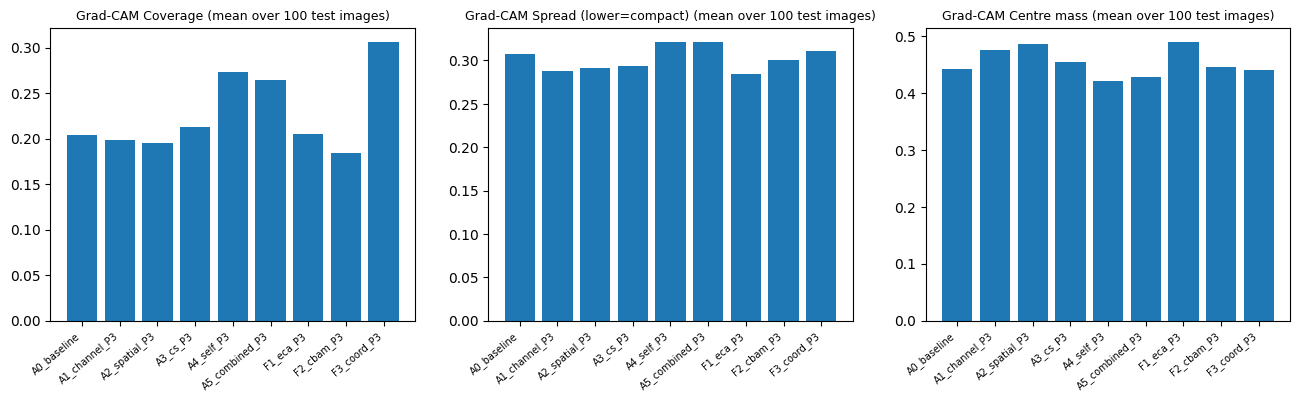
\includegraphics[width=\linewidth]{figs/gradcam_localisation.png}
\caption{Grad-CAM coverage, spread and centre mass (mean over 100 test images).}
\end{figure}

Over 100 test images the attention models change where the network looks only slightly: Grad-CAM coverage is 0.204 for the baseline, 0.185--0.212 for channel, spatial, Channel$\to$Spatial, ECA and CBAM, but larger for self-attention (0.273), combined (0.264) and coordinate attention (0.306), i.e.\ these distribute activation over a wider part of the image. Channel, spatial and ECA models are slightly more compact (spread 0.284--0.291 vs 0.308) and have slightly more mass in the central box (0.475--0.489 vs 0.442); self-attention and combined have less (0.420, 0.428). These shifts are small (3--5 points), so there is \textbf{no strong evidence of better foreground focus or background suppression}. For \emph{every} model, Grad-CAM mass in the central box is lower for wrongly classified images (e.g.\ baseline 0.382 vs 0.446 for correct; A3 0.373 vs 0.458) and coverage is also lower for wrong ones for every model, so incorrect predictions tend to come from less centred, more scattered evidence. Only 5--8 images per model are wrong, so this is indicative. The centre box is a proxy for the foreground, not a segmentation. Differences between shallow ($P_2$) and deep ($P_4$) attention are discussed in Section 29; consistency across images is high for the channel weights (0.997) and for the border-type spatial maps.


% ============================================================
\section*{31. Required Visualizations}
% ============================================================

The laboratory report must contain the following visualizations:

\begin{enumerate}

\item sample input images from all five classes;

\item training and validation accuracy curves;

\item training and validation loss curves;

\item confusion matrix;

\item feature map before attention;

\item channel-attention weights;

\item spatial-attention heatmap;

\item spatial-attention overlay;

\item self-attention response for the self-attention experiment;

\item feature map after attention;

\item baseline Grad-CAM;

\item Grad-CAM for at least one attention-based model;

\item attention maps at $P_2$, $P_3$, and $P_4$; and

\item at least one graphical comparison of the performances of different
attention mechanisms.

\end{enumerate}

% ============================================================
\section*{32. Recommended Visualization Layout}
% ============================================================

For one representative test image, students are encouraged to generate a
figure in the following format:

\[
\boxed{
\begin{array}{ccccc}
\text{Input}
&
\text{Baseline}
&
\text{Channel}
&
\text{Spatial}
&
\text{Channel+Spatial}
\\
&
\text{Grad-CAM}
&
\text{Grad-CAM}
&
\text{Attention Map}
&
\text{Grad-CAM}
\end{array}
}
\]

For students completing the additional attention comparison, the figure may
be extended to:

\[
\boxed{
\text{Input}
|
\text{Baseline}
|
\text{SE}
|
\text{ECA}
|
\text{CBAM}
|
\text{Self-Attention}
}
\]

using appropriate visualization methods.

% ============================================================
\section*{33. Required Experimental Analysis}
% ============================================================

The final report should contain three forms of analysis.

\subsection*{33.1 Quantitative Analysis}

Report:

\[
\boxed{
\text{Accuracy}
+
\text{Precision}
+
\text{Recall}
+
\text{Macro F1}
}
\]

\subsection*{33.2 Complexity Analysis}

Report:

\[
\boxed{
\text{Parameters}
+
\text{Inference Time}
}
\]

\subsection*{33.3 Qualitative Analysis}

Report:

\[
\boxed{
\text{Grad-CAM}
+
\text{Attention Maps}
+
\text{Visual Interpretation}
}
\]

Therefore, the overall evaluation should be:

\[
\boxed{
\text{Quantitative}
+
\text{Computational}
+
\text{Qualitative}
}
\]

% ============================================================
\section*{34. Experimental Protocol}
% ============================================================

To ensure fair comparison, all ablation experiments must use:

\begin{itemize}

\item identical training images;

\item identical validation images;

\item identical testing images;

\item identical random seed where possible;

\item identical image preprocessing;

\item identical augmentation;

\item identical backbone;

\item identical classifier;

\item identical optimizer;

\item identical batch size;

\item identical number of epochs;

\item identical learning-rate schedule;

\item identical fine-tuning procedure; and

\item identical evaluation metrics.

\end{itemize}

Only the experimental factor under investigation should change.

For example, when studying attention position:

\[
\boxed{
\text{Only Attention Position Should Change}
}
\]

and when studying attention type:

\[
\boxed{
\text{Only Attention Type Should Change}.
}
\]

% ============================================================
\section*{35. Minimum Mandatory Ablation Set}
% ============================================================

If laboratory time is limited, every student must complete at least the
following experiments:

\begin{enumerate}

\item Baseline pretrained ResNet50.

\item Channel attention at $P_3$.

\item Spatial attention at $P_3$.

\item Channel+Spatial attention at $P_3$.

\item Channel+Spatial attention at $P_2$.

\item Channel+Spatial attention at $P_4$.

\item Self-attention at $P_3$.

\item Grad-CAM comparison between baseline ResNet50 and one selected
attention model.

\item Spatial-attention visualization at $P_2$, $P_3$, and $P_4$.

\item Graphical comparison of the classification performance of the attention
models.

\end{enumerate}

This minimum set allows students to study:

\[
\boxed{\text{Attention Type}}
\]

and

\[
\boxed{\text{Attention Position}}.
\]

% ============================================================
\section*{36. Additional Student Exploration}
% ============================================================

Students interested in extended experimentation should select at least two
mechanisms from:

\[
\boxed{
\text{SE},
\quad
\text{ECA},
\quad
\text{CBAM},
\quad
\text{Coordinate Attention},
\quad
\text{Self-Attention}
}
\]

and integrate them with the same ResNet50 backbone.

Students should maintain the same:

\begin{itemize}

\item dataset split;

\item preprocessing;

\item augmentation;

\item optimizer;

\item epochs;

\item fine-tuning strategy; and

\item attention position.

\end{itemize}

The additional investigation should include both:

\[
\boxed{
\text{Quantitative Comparison}
}
\]

and

\[
\boxed{
\text{Qualitative Comparison}.
}
\]

% ============================================================
\section*{37. Questions Students Must Answer}
% ============================================================

\begin{enumerate}

\item What is the purpose of residual connections in ResNet50?

\item What does conv2\_x represent compared with conv5\_x?

\item Why does the spatial resolution decrease with network depth?

\item Why does the number of feature channels increase with network depth?

\item What is meant by low-level, intermediate, and high-level features?

\item What is the purpose of an attention mechanism?

\item What does channel attention attempt to learn?

\item What does spatial attention attempt to learn?

\item How is channel attention different from spatial attention?

\item Why can channel and spatial attention be used sequentially?

\item Why might channel attention behave differently at conv3\_x and
conv5\_x?

\item Why can spatial attention be useful at an intermediate ResNet stage?

\item Why is self-attention computationally expensive when the feature map
has high spatial resolution?

\item What happens to the size of the self-attention matrix when the spatial
resolution increases?

\item How does attention performance vary when the insertion position is
changed?

\item How does attention at $P_2$ differ visually from attention at $P_4$?

\item Does applying attention at multiple stages always improve
classification performance?

\item Does Channel$\rightarrow$Spatial attention behave differently from
Spatial$\rightarrow$Channel attention?

\item How does the spatial-attention kernel size influence the attention map?

\item How does SE attention differ from ECA attention?

\item How does CBAM combine channel and spatial attention?

\item How does self-attention differ from channel attention?

\item Does the attention mechanism with the largest number of parameters
necessarily provide the highest accuracy?

\item What is the difference between an internal attention map and Grad-CAM?

\item Why is Grad-CAM called a post-hoc explanation technique?

\item Does the attention model suppress irrelevant background regions?

\item Are the attention maps of correctly classified and incorrectly
classified images different?

\item Which flower classes benefit most from attention?

\item What information can be obtained from a confusion matrix that cannot
be obtained from overall accuracy alone?

\item Why is macro F1 useful in addition to accuracy?

\item What is meant by the accuracy--complexity trade-off?

\item What is meant by the F1--inference-time trade-off?

\item Why must every ablation study use the same dataset split?

\item Why must the same training protocol be maintained when comparing
different attention mechanisms?

\item What conclusions can be drawn from the Grad-CAM comparison?

\end{enumerate}


\subsection*{Observations: Answers to the Questions}
\begin{enumerate}
\item \textbf{Residual connections} add the block input to its output ($y=F(x)+x$); the identity path lets gradients reach early layers, avoids degradation in very deep networks and lets blocks learn only a residual correction. ResNet50 has 16 of them.
\item \textbf{conv2\_x vs conv5\_x:} conv2\_x ($56\times56\times256$) holds low-level features (edges, colours, textures) with a small receptive field; conv5\_x ($7\times7\times2048$) holds high-level, class-discriminative semantic features with a large receptive field.
\item \textbf{Resolution decreases} because the first block of conv3\_x, conv4\_x and conv5\_x uses stride 2, enlarging the receptive field and reducing computation while building more abstract features.
\item \textbf{Channels increase} to encode the richer and more varied patterns needed at higher levels and to compensate for lost spatial detail.
\item \textbf{Levels:} low = edges, colour blobs, simple textures; intermediate = repeated patterns, petal arrangements, flower parts; high = whole-object structure and class semantics (daisy vs tulip).
\item \textbf{Purpose of attention:} input-dependent re-weighting that emphasises informative channels/locations and suppresses irrelevant ones.
\item \textbf{Channel attention} learns which channels matter (one weight per channel from a global descriptor).
\item \textbf{Spatial attention} learns which locations matter (one weight per position, shared by all channels).
\item \textbf{Difference:} channel attention is spatially uniform (``what''); spatial attention is channel-uniform (``where'').
\item \textbf{Sequential use} is possible because they are complementary and cheap: the spatial map is computed from already channel-refined features (as in CBAM).
\item \textbf{Channel attention at conv3\_x vs conv5\_x:} conv3\_x channels (512) are mid-level pattern detectors, conv5\_x channels (2048) are semantic; the module is also 16$\times$ larger at conv5\_x ($526{,}563$ vs $33{,}411$ parameters). In our runs B2 (0.9328) and B4 (0.9365) differ by less than one standard error.
\item \textbf{Spatial attention at an intermediate stage} works on a map ($28\times28$ or $14\times14$) that still resolves flower vs background while the features are already meaningful; $P_1$ is too low-level (and costly) and $P_4$ too coarse. In our results $P_3$ is best and $P_1$ clearly worse.
\item \textbf{Self-attention is expensive at high resolution} because it builds an $N\times N$ matrix with $N=HW$ (3136$^2\approx9.8$ M entries per image at $P_1$).
\item \textbf{Matrix size} grows quadratically with $N$: doubling $H$ and $W$ gives 4$\times$ more positions and a 16$\times$ larger matrix (9.83 M at $P_1$ vs 38{,}416 at $P_3$).
\item \textbf{Position changes performance:} Channel$\to$Spatial accuracy is 0.9129 ($P_1$), 0.9328 ($P_2$), 0.9437 ($P_3$), 0.9365 ($P_4$).
\item \textbf{$P_2$ vs $P_4$ visually:} a thin bottom-edge band at $P_2$ versus a compact lower-right blob at $P_4$; both leave the flower regions at about 1, so the expected edge-vs-semantic distinction is not visible (Section 29).
\item \textbf{Multiple stages:} no; $P_3{+}P_4$ ($-1.5$ points) and $P_2{+}P_3{+}P_4$ ($-3.6$ points) were worse than $P_3$ alone.
\item \textbf{Order:} Channel$\to$Spatial 0.9437 vs Spatial$\to$Channel 0.9328, a difference inside the noise level; maps correlate 0.93--0.99.
\item \textbf{Kernel size:} accuracy rises with $k$ (0.9056, 0.9310, 0.9437), but the maps do not show clearly richer context (3$\times$3 maps are the most varied, 5$\times$5 and 7$\times$7 are nearly saturated).
\item \textbf{SE vs ECA:} SE uses GAP $\to$ bottleneck MLP (reduction $r$, $\approx2C^2/r$ parameters, every channel interacts with all others); ECA drops the reduction and applies a 1-D convolution of adaptive kernel size over neighbouring channels (5 parameters at $C=1024$).
\item \textbf{CBAM} applies a channel gate (average- and max-pooled descriptors through a shared MLP, summed, sigmoid) followed by a spatial gate (channel-wise mean and max maps, $7\times7$ convolution, sigmoid).
\item \textbf{Self-attention vs channel attention:} self-attention relates every spatial position to every other (long-range, content-dependent, $N\times N$) and outputs a weighted sum of values; channel attention only rescales channels from a global descriptor.
\item \textbf{Largest module = highest accuracy?} No: self-attention (1.31 M) and the combined module (1.44 M) are not better than the 132 k-parameter Channel$\to$Spatial module (0.9437), and the combined module is lower (0.9274).
\item \textbf{Internal map vs Grad-CAM:} the internal map is computed by the module in the forward pass and changes the prediction; Grad-CAM is computed afterwards from gradients of a class score and does not change the model.
\item \textbf{Post-hoc:} Grad-CAM needs a finished prediction and a backward pass on a trained model; it explains the network but is not part of its computation.
\item \textbf{Background suppression:} the spatial gates suppress mainly the image border (bottom band/corner) rather than the background clutter, and Grad-CAM differences are small (Section 30): at most weak evidence.
\item \textbf{Correct vs incorrect:} the internal spatial maps look alike for both; Grad-CAM centre-box mass and coverage are lower for incorrect predictions in all nine models (e.g.\ baseline 0.382 vs 0.446).
\item \textbf{Classes that benefit most:} tulips (F1 $+0.071$ with A3 and the largest average gain) and dandelion (recall 0.830 $\to$ 1.000); roses does not benefit.
\item \textbf{Confusion matrix vs accuracy:} it shows which classes are confused in which direction (e.g.\ the baseline's sink class is tulips; attention removed dandelion$\to$tulips but created dandelion-directed errors), per-class recall/precision, and where gains occur, all hidden by one accuracy value.
\item \textbf{Macro F1} averages the per-class F1 with equal weight, so weak classes (roses, tulips) are not masked by large ones and precision and recall are balanced; the classes are slightly imbalanced (135 vs 95 test images).
\item \textbf{Accuracy--complexity trade-off:} accuracy gained per additional parameter/FLOP; here the 99-parameter spatial module gives nearly the whole gain, so extra parameters bought nothing.
\item \textbf{F1--inference-time trade-off:} F1 gained per extra millisecond per image; here latency differences ($\pm0.5$ ms) are within measurement noise, so GFLOPs ($+0.60$ only for self-attention) is the better cost measure.
\item \textbf{Same split} so differences come from the model and not from a different test set (one accuracy has a 1.28-point standard error).
\item \textbf{Same protocol} (optimiser, learning rates, epochs, augmentation, seed, fine-tuning) because these influence accuracy as much as the module; only the factor under study may change.
\item \textbf{Grad-CAM conclusions:} for correct images baseline and attention models look at the same flower; differences appear for wrongly classified images, where the predicted class follows the region highlighted; over 100 images the changes are small (coverage and centre mass shift by 0.02--0.1), so Grad-CAM supports ``similar focus, somewhat different coverage'' but not ``clearly better localisation''.
\end{enumerate}


% ============================================================
\section*{38. Observations to be Recorded}
% ============================================================

Students should record the following during experimentation:

\begin{enumerate}

\item Input and output feature dimensions for each attention module.

\item Training accuracy.

\item Validation accuracy.

\item Testing accuracy.

\item Training loss.

\item Validation loss.

\item Macro precision.

\item Macro recall.

\item Macro F1-score.

\item Number of trainable parameters.

\item Total number of model parameters.

\item Average inference time.

\item Confusion matrix.

\item Channel-attention weights.

\item Spatial-attention maps.

\item Self-attention responses.

\item Grad-CAM maps.

\item Attention maps for different insertion positions.

\end{enumerate}


\subsection*{Where the Observations Are Recorded}
Observation 1 (feature dimensions) is recorded in Section 13; observations 2--6 and 10--12 are in the observation sheet in Section 24 and the complexity table in Section 23; macro precision, recall and F1 are in the tables of Sections 14--19 and 23; confusion matrices are in Section 25; channel-attention weights in Section 28.1; spatial maps in Sections 28.2 and 29; self-attention responses in Section 28.3; Grad-CAM maps in Section 27; and attention maps for different insertion positions in Section 29.


% ============================================================
\section*{39. Suggested Laboratory Report Structure}
% ============================================================

The laboratory report may be organized as follows:

\begin{enumerate}

\item \textbf{Aim}

\item \textbf{Dataset Description}

\item \textbf{ResNet50 Architecture}

\item \textbf{Attention Mechanisms}

\item \textbf{Proposed Experimental Architecture}

\item \textbf{Experimental Setup}

\item \textbf{Attention-Type Ablation}

\item \textbf{Attention-Position Ablation}

\item \textbf{Performance Results}

\item \textbf{Complexity Analysis}

\item \textbf{Training and Validation Graphs}

\item \textbf{Confusion Matrix Analysis}

\item \textbf{Grad-CAM Analysis}

\item \textbf{Internal Attention-Map Analysis}

\item \textbf{Qualitative Comparison}

\item \textbf{Additional Attention-Mechanism Comparison}

\item \textbf{Discussion}

\item \textbf{Conclusion}

\end{enumerate}

% ============================================================
\section*{40. Discussion Guidelines}
% ============================================================

Students should not merely reproduce numerical results.

The discussion should explain:

\begin{itemize}

\item why a particular attention mechanism produced a change in performance;

\item how attention location influences feature refinement;

\item how feature resolution changes attention behavior;

\item how model complexity changes with different mechanisms;

\item whether performance improvements justify additional computational cost;

\item whether attention maps correspond to meaningful object regions;

\item whether attention helps suppress the background;

\item whether attention behaves differently for incorrect predictions; and

\item whether quantitative and qualitative observations support each other.

\end{itemize}

Students should avoid making conclusions based on a single image.

Qualitative observations should preferably be based on several representative
test images.


\subsection*{Observations: Discussion}
\textbf{Why did attention change performance?} Three of the six attention-type models (spatial, Channel$\to$Spatial, self-attention) improved the baseline by about four points and the channel-only modules by 1--2 points. Because the channel weights are almost input-independent and the spatial maps pass most of the image unchanged, the improvement is unlikely to come from careful selection of flower regions; plausible contributors are re-scaling of the features entering conv5\_x (which is fine-tuned), reduced late overfitting (the baseline's validation accuracy fell after epoch 7) and run-to-run variation. A multi-seed study would be needed to separate these.
\textbf{Position and resolution.} The best position ($P_3$) has moderate resolution and meaningful features; $P_1$ is both less accurate and most expensive. \textbf{Complexity.} Only self-attention increases GFLOPs noticeably and its cost scales with $(HW)^2$, which is why it belongs at $P_3$/$P_4$. \textbf{Do improvements justify cost?} For the spatial and Channel$\to$Spatial modules yes (negligible cost); for the combined and multi-stage models no. \textbf{Do quantitative and qualitative results agree?} Partly: both show that attention changes behaviour only modestly (small Grad-CAM shifts), while accuracy changes by up to 4 points; the internal maps reveal border-type spatial gating and nearly static channel gating, which explains why strong ``semantic'' attention was not observed.


\subsection*{Observations: Limitations}
(i) Each configuration was trained once (seed 42); differences below about 2.5 points are not reliable. (ii) Last-epoch weights were used without checkpoint selection. (iii) Inference times are noisy; peak-memory readings were contaminated and are not reported. (iv) The centre-box measure is a proxy for the foreground. (v) Qualitative statements rest on five images (plus 100-image proxies); one of the ``wrong'' images contains no prominent flower.


% ============================================================
\section*{41. Expected Outcome}
% ============================================================

At the end of the experiment, students should understand that an attention
mechanism is not an isolated module whose behavior is independent of the
backbone.

Its effectiveness depends on:

\[
\boxed{
\begin{aligned}
\text{Attention Effectiveness}
={}&
\text{Attention Type}\\
&+
\text{Attention Position}\\
&+
\text{Feature Resolution}\\
&+
\text{Feature Semantics}\\
&+
\text{Model Complexity}.
\end{aligned}
}
\]

Students should also understand that classification performance alone does
not provide a complete explanation of an attention mechanism.

A comprehensive analysis should therefore combine:

\[
\boxed{
\text{Classification Performance}
}
\]

with

\[
\boxed{
\text{Computational Complexity}
}
\]

and

\[
\boxed{
\text{Qualitative Visualization}.
}
\]

Therefore:

\[
\boxed{
\text{Complete Attention Analysis}
=
\text{Quantitative}
+
\text{Computational}
+
\text{Qualitative}
}
\]

The final conclusions must be based on the student's experimental results
rather than on assumptions about which attention mechanism should perform
best.



\subsection*{Observations: Conclusion}
Under an identical protocol, attention inserted after conv4\_x of a pretrained ResNet50 raised test accuracy on \texttt{tf\_flowers} from 0.9002 to as much as 0.9437 (Channel$\to$Spatial; spatial-only and self-attention 0.9419), with macro F1 from 0.9033 to 0.9420. The best position is $P_3$; attention at $P_1$ helps little, and attention at several stages, a combined C+S+SA module or a larger parameter budget did not help. The order of channel and spatial attention has no reliable effect, and larger spatial kernels gave higher accuracy without clearly richer maps. Computationally only self-attention is noticeably heavier (+0.60 GFLOPs, +1.31 M parameters), while spatial attention with 99 parameters performs equally well. Internal maps show nearly static channel weights and border-dominated spatial gates, and Grad-CAM shows similar focus for baseline and attention models with small changes in coverage, so the gains cannot be attributed to markedly better flower localisation. The overall conclusion rests on a single-seed study and should be confirmed with repeated runs.


\clearpage
% ============================================================
\section*{42. References}
% ============================================================

\begin{enumerate}

\item
K. He, X. Zhang, S. Ren, and J. Sun,
``Deep Residual Learning for Image Recognition,''
\textit{Proceedings of the IEEE Conference on Computer Vision and Pattern
Recognition (CVPR)}, pp. 770--778, 2016.

\item
J. Hu, L. Shen, S. Albanie, G. Sun, and E. Wu,
``Squeeze-and-Excitation Networks,''
\textit{IEEE Transactions on Pattern Analysis and Machine Intelligence},
vol. 42, no. 8, pp. 2011--2023, 2020.

\item
S. Woo, J. Park, J.-Y. Lee, and I. S. Kweon,
``CBAM: Convolutional Block Attention Module,''
\textit{Proceedings of the European Conference on Computer Vision (ECCV)},
pp. 3--19, 2018.

\item
Q. Wang, B. Wu, P. Zhu, P. Li, W. Zuo, and Q. Hu,
``ECA-Net: Efficient Channel Attention for Deep Convolutional Neural
Networks,''
\textit{Proceedings of the IEEE/CVF Conference on Computer Vision and Pattern
Recognition (CVPR)}, pp. 11534--11542, 2020.

\item
Q. Hou, D. Zhou, and J. Feng,
``Coordinate Attention for Efficient Mobile Network Design,''
\textit{Proceedings of the IEEE/CVF Conference on Computer Vision and Pattern
Recognition (CVPR)}, pp. 13713--13722, 2021.

\item
A. Vaswani et al.,
``Attention Is All You Need,''
\textit{Advances in Neural Information Processing Systems},
vol. 30, 2017.

\item
R. R. Selvaraju, M. Cogswell, A. Das, R. Vedantam,
D. Parikh, and D. Batra,
``Grad-CAM: Visual Explanations from Deep Networks via
Gradient-Based Localization,''
\textit{Proceedings of the IEEE International Conference on Computer Vision
(ICCV)}, pp. 618--626, 2017.

\item
TensorFlow Documentation:
\url{https://www.tensorflow.org/}

\item
Keras Documentation:
\url{https://keras.io/}

\item
TensorFlow Datasets:
\url{https://www.tensorflow.org/datasets}

\end{enumerate}

% ============================================================
% END DOCUMENT
% ============================================================

\end{document}
